% Include only the SI item label in the subsection heading. Use the \nameref{label} command to cite SI items in the text.
\section{Data Collection Methodology}
\label{sec:data_collection_methodology}
The Twitter Search
API \cite{Twitter_API}
%\footnote{\url{http://dev.twitter.com} (Accessed: August 25, 2015)} 
retrieves recent tweets that can possibly date back to the last 6
to 9 days.  The Search API retrieves an indexing of the recent tweets
but is not guaranteed to be a comprehensive retrieval. Had we
carried out the project by obtaining a batch of news events from the
past, the searches will most certainly fail to retrieve the early
tweets.  It is very essential that the tweet collection process be in real
time and that we begin retrieving the
tweets for a particular event as soon as the event breaks out.  Recall that we
want to analyze if the early tweets contain any signals that
differentiate the high-impact events from the rest. 


% Please add the following required packages to your document
% preamble: \usepackage{booktabs}
\begin{table}[h]
  \centering
  \begin{tabular}{@{}lllll@{}}
    \toprule
    \textbf{News events' property} & \textbf{Minimum} & \textbf{Mean} & \textbf{Median} & \textbf{Maximum} \\ \midrule
    \# of posts & $1,000$ & $8,254$ & $2,474$ & $510,920$ \\
    \# of keywords & $2$ & $3.77$ & $3$ & $39$ \\ 
    Event duration (hours) & $0.12$ & $20.93$ & $7.46$ & $190.43$ \\ \bottomrule
  \end{tabular}
  \caption{\bf High-level description of the dataset of news events.} \label{table:dataset-stats}

\end{table}

We have collected $5,234$ news events gathered from news headlines.
The overall number of tweets obtained for all the collected events is
$43,256,261$. Table~\ref{table:dataset-stats} shows a high level
description of the dataset (the full
  dataset is available in
  \url{http://dcc.uchile.cl/~mquezada/breakingnews/).}.

\subsection{Collecting the Tweets}
\label{sec:collecting_the_data}
At a high level, the data collection process entails detecting pairs
of keywords from the most recent hourly batch of news headlines (the
pairs of keywords are meant to describe the events succinctly), and
then searching for tweets using the pairs of keywords as queries.
Figure~\ref{fig:data_collection_1} represents the high-level flowchart
of the data collection process. A summary of this process is described
in Algorithm~\ref{alg:data_collection}. We merge the search results of
`similar' queries every 24 hours and form the tweets set for an event.
We obtained the hourly batch of headlines from the news media accounts
on Twitter. The accounts are verified accounts on
Twitter (verified accounts on Twitter establish authenticity
  of identity of key individuals and organizations).



{\footnotesize
  \begin{longtable}{lll}
    \toprule
    \textbf{Twitter Account} & \textbf{Name} & \textbf{Location} \\
    \midrule
    \endfirsthead
    \multicolumn{3}{l}%
    {\tablename\ \thetable\ -- \textit{Continued from previous page}} \\
    \toprule
    \textbf{Twitter Account} & \textbf{Name} & \textbf{Location} \\
    \midrule
    \endhead
    \hline \multicolumn{3}{l}{\textit{Continued on next page}} \\
    \endfoot
    \bottomrule
    \endlastfoot

    breakingnews     &  Breaking News         &  Global                      \\
    cnnbrk           &  CNN Breaking News     &  Everywhere                  \\
    cnn              &  CNN                   &                              \\
    nytimes          &  The New York Times    &  New York City               \\
    bbcbreaking      &  BBC Breaking News     &  London, UK                  \\
    theeconomist     &  The Economist         &  London                      \\
    skynewsbreak     &  Sky News Newsdesk     &  London, UK                  \\
    reuters          &  Reuters Top News      &  Around the world            \\
    wsjbreakingnews  &  WSJ Breaking News     &  New York, NY                \\
    foxnews          &  Fox News              &  U.S.A.                      \\
    msnbc\_breaking   &  msnbc.com Breaking    &                              \\
    skynews          &  Sky News              &  London, UK                  \\
    nbcnews          &  NBC News              &  New York, NY                \\
    cbsnews          &  CBS News              &  New York, NY                \\
    bbcworld         &  BBC News (World)      &  London, UK                  \\
    abc              &  ABC News              &  New York, NY                \\
    bbcnews          &  BBC News (UK)         &  London                      \\
    ap               &  The Associated Press  &  Global                      \\
    telegraphnews    &  Telegraph News        &  London, UK                  \\
    breakingnewsuk   &  Breaking News UK      &  London                      \\
    channel4news     &  Channel 4 News        &  Weekdays at 7 on Channel 4  \\
    twcbreaking      &  TWC Breaking          &  Atlanta, GA                 \\
    washingtonpost   &  Washington Post       &  Washington, D.C.            \\
    yahoonews        &  Yahoo News            &  Santa Monica, Calif.        \\
    breakingpol      &  Breaking Politics     &  Global                      \\
    nydailynews      &  New York Daily News   &  New York City               \\
    ajenglish        &  Al Jazeera English    &  Doha, Qatar                 \\
    usatoday         &  USA TODAY             &  USA TODAY HQ, McLean, Va.   \\
    wsj              &  Wall Street Journal   &  New York, NY                \\
    guardiannews     &  Guardian news         &  London                      \\
    bloombergnews    &  Bloomberg News        &  New York and the World      \\
    abcworldnews     &  ABC World News        &  New York                    \\
    nypost           &  New York Post         &  New York, NY                \\
    msnbc            &  msnbc                 &                              \\
    nbcnightlynews   &  NBC Nightly News      &  New York                    \\
    huffingtonpost   &  Huffington Post       &                              \\
    rt\_com           &  RT                    &                              \\
    abcnews          &  ABC News              &  Australia                   \\
    latimes          &  Los Angeles Times     &  Los Angeles, CA             \\
    googlenews       &  Google News           &  Mountain View, CA           \\
    cnnlive          &  CNN Live              &  Everywhere                  \\
    newshour         &  NewsHour              &  Arlington, VA               \\
    guardian         &  The Guardian          &  London                      \\
    afp              &  Agence France-Presse  &  France                      \\
    independent      &  The Independent       &  London, United Kingdom      \\
    ndtv             &  NDTV                  &  India                       \\
    cp24             &  CP24                  &  Toronto                     \\
    reuterslive      &  Reuters Live          &  Global                      \\
    bostonglobe      &  The Boston Globe      &  Boston, MA                  \\
    foxnewsalert     &  Fox News Alert        &  New York, NY                \\
    ft               &  Financial Times       &  London                      \\
    jerusalem\_post   &  The Jerusalem Post    &  Israel                      \\
    bbcnewsus        &  BBC News US           &  Washington DC               \\
    foxheadlines     &  Fox News              &  New York, NY                \\
    forbes           &  Forbes                &  New York, NY                \\
    thetimes         &  The Times of London   &  London                      \\
    usnews           &  U.S. News             &  Washington, DC\\

    \caption[List of news accounts.]{\textbf{List of news account. The
        first column is the Twitter account. It can be accessed in a
        browser at \texttt{http://twitter.com/accountname}. The second
        and third columns were obtained from each account's page.}}

\end{longtable}
}

In Algorithm~\ref{alg:data_collection}, the goal of the {\tt
  detect\_keywords()} module is to produce pairs of keywords that
coherently, and succinctly describes an event. Inspired by the data
mining concept of mining frequent itemsets \cite{Tan_Steinbach_Kumar},
we develop an algorithm which identifies the most commonly occurring
keyword groups (or item sets) in the headlines. From the item sets, we
pick the most common keyword pairs. The algorithm is described in
Algorithm~\ref{alg:detect_keywords}. This algorithm finds string
intersections between headlines ({\tt intersect()} in
Line~\ref{alg:line:intersect} returns the number of words present in
both $s_a$ and $s_b$). If the common set of words has sufficient
Jaccard similarity to any of the existing item sets, then the common
set of words are added to that item set. If not, a new item set is
created (Line~\ref{alg:line:create}). During the process of
identifying the most commonly occurring item sets, we also track how
many times each keyword has been added to an item set, namely, the
score of the keyword. The score of each item set is the average of the
scores of its
keywords. The module \texttt{addOne()} adds one to the score
of every keyword in the input set.%\footnote{The module {\tt addOne() adds 1 to the score of
% every keyword in the input set.}}.
Once the item sets have been identified, we select the top 2 keywords
from each of the top six item sets and use them for searches. We
preprocess the headlines to remove duplicates, stopwords, punctuation,
convert everything to lower case, and subject the text through the
process of stemming.

We made the choice of selecting 2 keywords since having a single
keyword maybe not define an event accurately. For example, the keyword
\{obama\} could retrieve tweets about any event related to Obama.
However, a keyword \emph{pair} like \{obama, syria\} describes the
event more accurately.  Having more than two keywords may impose
too much of a restriction on the query, leading to little
or no tweets in the retrieval.
%\footnote{Having more than two keywords may
%  impose too much of a restriction on the query, leading to little or
%  no tweets in the retrieval.}.

The Twitter Search API imposes several restrictions on the number of
searches that can be performed in a given time duration.
% In order to circumvent this restriction and capture as many tweets
% as we possibly can,
We produce six search threads to perform searches, one for each
keyword pair. All in all, with $\tau = 60$ minutes in
Figure~\ref{fig:data_collection_1}, six new pairs of keywords are
discovered from the most recent batch of headlines, and then we query
for tweets in the Twitter Search API using these keywords over the
next one hour.

We make some notes about the data collection methodology. Firstly,
there is a temporal sensitivity to the data collection methodology.
For example, one of the keyword pairs obtained as soon the Malaysian
airlines jet disappeared was \{plane,missing\}. Although this keyword
pair does not specifically refer to the Malaysian airlines jet, it is
likely that the tweets retrieved from searching for this pair will
indeed be about the Malaysian airlines plane that went missing, since
the search is performed as and when the event breaks out. Secondly,
Algorithm~\ref{alg:detect_keywords} may return multiple pairs of
keywords (possibly different pairs) describing the same event. Some
pair examples of keywords produced when there was a bomb threat at
Harvard University in December 2013 were \{harvard, evacuated\},
\{harvard, explosives\}, etc. How do we merge the keyword pairs which
belong to the same event? In order to address this, we collect all the
pairs obtained in the past $24$ hours, and build a graph with keywords
as nodes, and keyword pairs (as obtained from Algorithm
{\ref{alg:detect_keywords}}) as edges. We then discover the connected
components of this graph, and treat each connected component as an
``event".  For the rest of the document, the terms \emph{connected component}
and \emph{event} are used interchangeably.  Both of them refer to the definition
of \emph{event} in the main article.
%\footnote{For the rest of the document, the terms
%  \emph{connected component} and \emph{event} are used
%  interchangeably. Both of them refer to the definition of
%  \emph{event} given in the main article.}. 
The set of tweets obtained
by merging the tweets from each of the keyword pairs is the set of
messages associated with the event. Figure
\ref{fig:connected_components} is an example component formed on
December 16, 2013. It illustrates the merge of smaller keyword pairs
into larger components for two events. One was the bomb threat at
Harvard University, and the other was about the attack on police in
the Xinjiang province in China.

\begin{figure}
  
\includegraphics[width=\textwidth]{figures_SI/Pictures_and_Drawings/data_collection_1}
  \caption{\textbf{This figure illustrates the high level data
      collection process. Headlines are collected every hour, and $6$
      keyword pairs are chosen to search for tweets. These keyword
      pairs are detected with the goal of concisely representing
      queries for an event.}}
  \label{fig:data_collection_1}
\end{figure}

\begin{algorithm}
  \caption{{\tt data\_collection()}}
  \label{alg:data_collection}
  \begin{algorithmic}[1]
    \REQUIRE stream of headlines. \\
    \ENSURE data structures $\{\H_1, \H_2, \ldots \}$, with $\H.keywords$ = keyword pair, and $\H.tweets$ = set of tweets\\
    \STATE $i \leftarrow 0$, $j \leftarrow 0$ \\
    \LOOP
    \STATE $\mathcal{S} \leftarrow$ headlines for hour-$i$ \\
    \STATE $keyPairs \leftarrow$ {\tt detect\_keywords$(\mathcal{S})$}
    \COMMENT{$keyPairs$ is a list of keyword pairs.} \FOR{$k = 0$ to
      {\tt len($keyPairs$)$-1$}}
    \STATE $\H_j.keywords \leftarrow keyPairs[k]$ \\
    \STATE $\H_j.tweets \leftarrow $search$(\H_j.keywords)$
    \COMMENT{using Twitter Search API} \STATE $j \leftarrow j+1$
    \ENDFOR
    \STATE $i \leftarrow i+1$
    \ENDLOOP
  \end{algorithmic}
\end{algorithm}


\begin{algorithm}
  \caption{\tt{detect\_keywords()}}
  \label{alg:detect_keywords}
  \begin{algorithmic}[1]
    \REQUIRE A set of $M$ sets of words, $\ess= \{H_1,H_2, \ldots,
    H_M\}$, positive integers $k, \eta$ \ENSURE $k$ sets of keywords,
    $G = (\I_1,\I_2,\ldots,\I_{k})$ \STATE $\I_i \leftarrow \emptyset$
    for $i = 1,2,
    \ldots,k$ %\COMMENT{Initialize item sets to empty sets}
    \STATE $score_i \leftarrow$ empty dictionary for $i = 1, 2,
    \ldots,k$ %\COMMENT{Initialize keyword set scores to $1$}
    \STATE $i \leftarrow 1$ \FOR{every pair of headlines $\{H_a, H_b\}
      \in \ess$ such that $|H_a \cap H_b| \geq \eta$} \STATE $\G
    \leftarrow H_a \cap H_b$
    \label{alg:line:intersect} %\COMMENT{$\G$ is the set of common words of $H_a$ and $H_b$}
    \STATE $j \leftarrow \operatorname{arg\,max}_j |\I_j \cap \G|$
    \IF{$|\I_j \cap \G| \geq \eta$} \STATE $\I_j \leftarrow \I_j \cap
    \G$ \STATE $score_{j}[w] \leftarrow score_{j}[w] + 1$ for all $w
    \in \I_j$ \ELSE \STATE $\I_i \leftarrow
    \G$ \label{alg:line:create} \STATE $score_{i}[w] \leftarrow 1$ for
    all $w \in \I_i$ \STATE $i \leftarrow i + 1$
    \ENDIF
    \ENDFOR
    \STATE $total\_score_i \leftarrow \sum_{w \in \I_i} score_{i}[w]$
    for $i = 1,2,\ldots,k$ \RETURN $G \leftarrow (\I_i$ sorted by
    $total\_score_i)$
  \end{algorithmic}
\end{algorithm}

\subsection{Cleaning the Data}
There were a few issues which we faced during data collection. We
explain and address the issues here.
\subsubsection{Special Stopwords:  Articulation Words}
A problem that arose during the data collection was that, sometimes
unrelated events were joined together with keywords that was common to
both events.  

Typical stopwords such as ``the" and ``a" were removed during preprocessing
the news headlines. But as it turns out, there are other words
which occur quite commonly in news headlines. For example, words like
``watch'', ``live'', or ``update'' are common to express things like
``watch this video'', ``we are live on TV'', or to update a previous
headline with more information about it. By having sharing commonality
between different
events (for example:  ``Watch Jim Harbaugh's press conference
live" \cite{Jim}, and ``WATCH LIVE: Of the 48 people being monitored for
contact with Dallas patient, no one is showing any symptoms'' \cite{dallas_patient})
%(for example: ``Watch Jim Harbaugh's press conference
%live''\footnote{\url{https://twitter.com/49ers/status/519202023628374016}
%(Accessed: August 25, 2015)}



%and ``WATCH LIVEi: Of the 48 people being monitored for contact with
%Dallas patient, no one is showing any
%symptoms''\footnote{\url{https://twitter.com/PzFeed/status/519203692898435072}
%(Accessed: August 25, 2015)},
they could possibly incorrectly connect events which in reality are
unrelated.  We call such words
\emph{articulation words} in the sense that if they appear as keywords
after processing a group of headlines, then when joining the searches
together, those words would join unrelated events.  We now delve into
understanding how and when these words occur, and how to subsequently
identify and remove them in the preprocessing step, just as we would a
stopword.

It is well known that \emph{tf-idf} \cite{Jones72astatistical} is a statistic of a word that
indicates how important that word is in a given document.  Intuitively, if a word appears
in all the documents, then its statistic is generally low in all the documents.  However,
if the word appears in very few documents, its statistic in those documents is fairly high,
indicating that the word is somehow representative of the content of the document.
It turns out the articulation words do not occur often enough for them to be detected by
regular \emph{tf-idf}, but do occur enough
times for them to falsely relate several unrelated events together. To
identify a group of those keywords, we used a modified \emph{tf-idf}
to detect them from the headlines.

The modified version of \emph{tf-idf}, what we refer as
\emph{maxtf-idf}, is meant to assign more weight to the terms that are
frequent in any document. For instance, \emph{tf-idf} of a term in a
document tries to assign a weight related to how ``rare'' that term is
in the whole collection, and how frequent the term is in that document,
thus indicating how representative is the term in the document. On the
other hand, what we want is to put a higher weight in a term, if that term is more
frequent in any document, relative to the frequency in the current
document. With that in mind, we want to identify terms that might be
``adding noise'' to the corpus and hence end up joining unrelated
events together.

The definition of \emph{maxtf} is as follows:

\begin{equation}
  \text{maxtf}(t,d,D) = 0.5 + \frac{0.5 + max\{f(t,d') : d' \in D\}}{max\{f(w,d) : w \in d\}}
\end{equation}

and for \emph{idf}, the usual formula:

\begin{equation}
  \text{idf}(t,D) = \log\frac{N}{|\{d \in D : t \in d\}|}
\end{equation}

where $t$ is a term, $d$ is a document, and $D$ is the corpus of all
documents. In this case, we set $t$ as a keyword, $d$ as the set of
keywords of one hour of a given day, and $D$ the set of documents of
that day.

\begin{figure}
  \begin{center}
    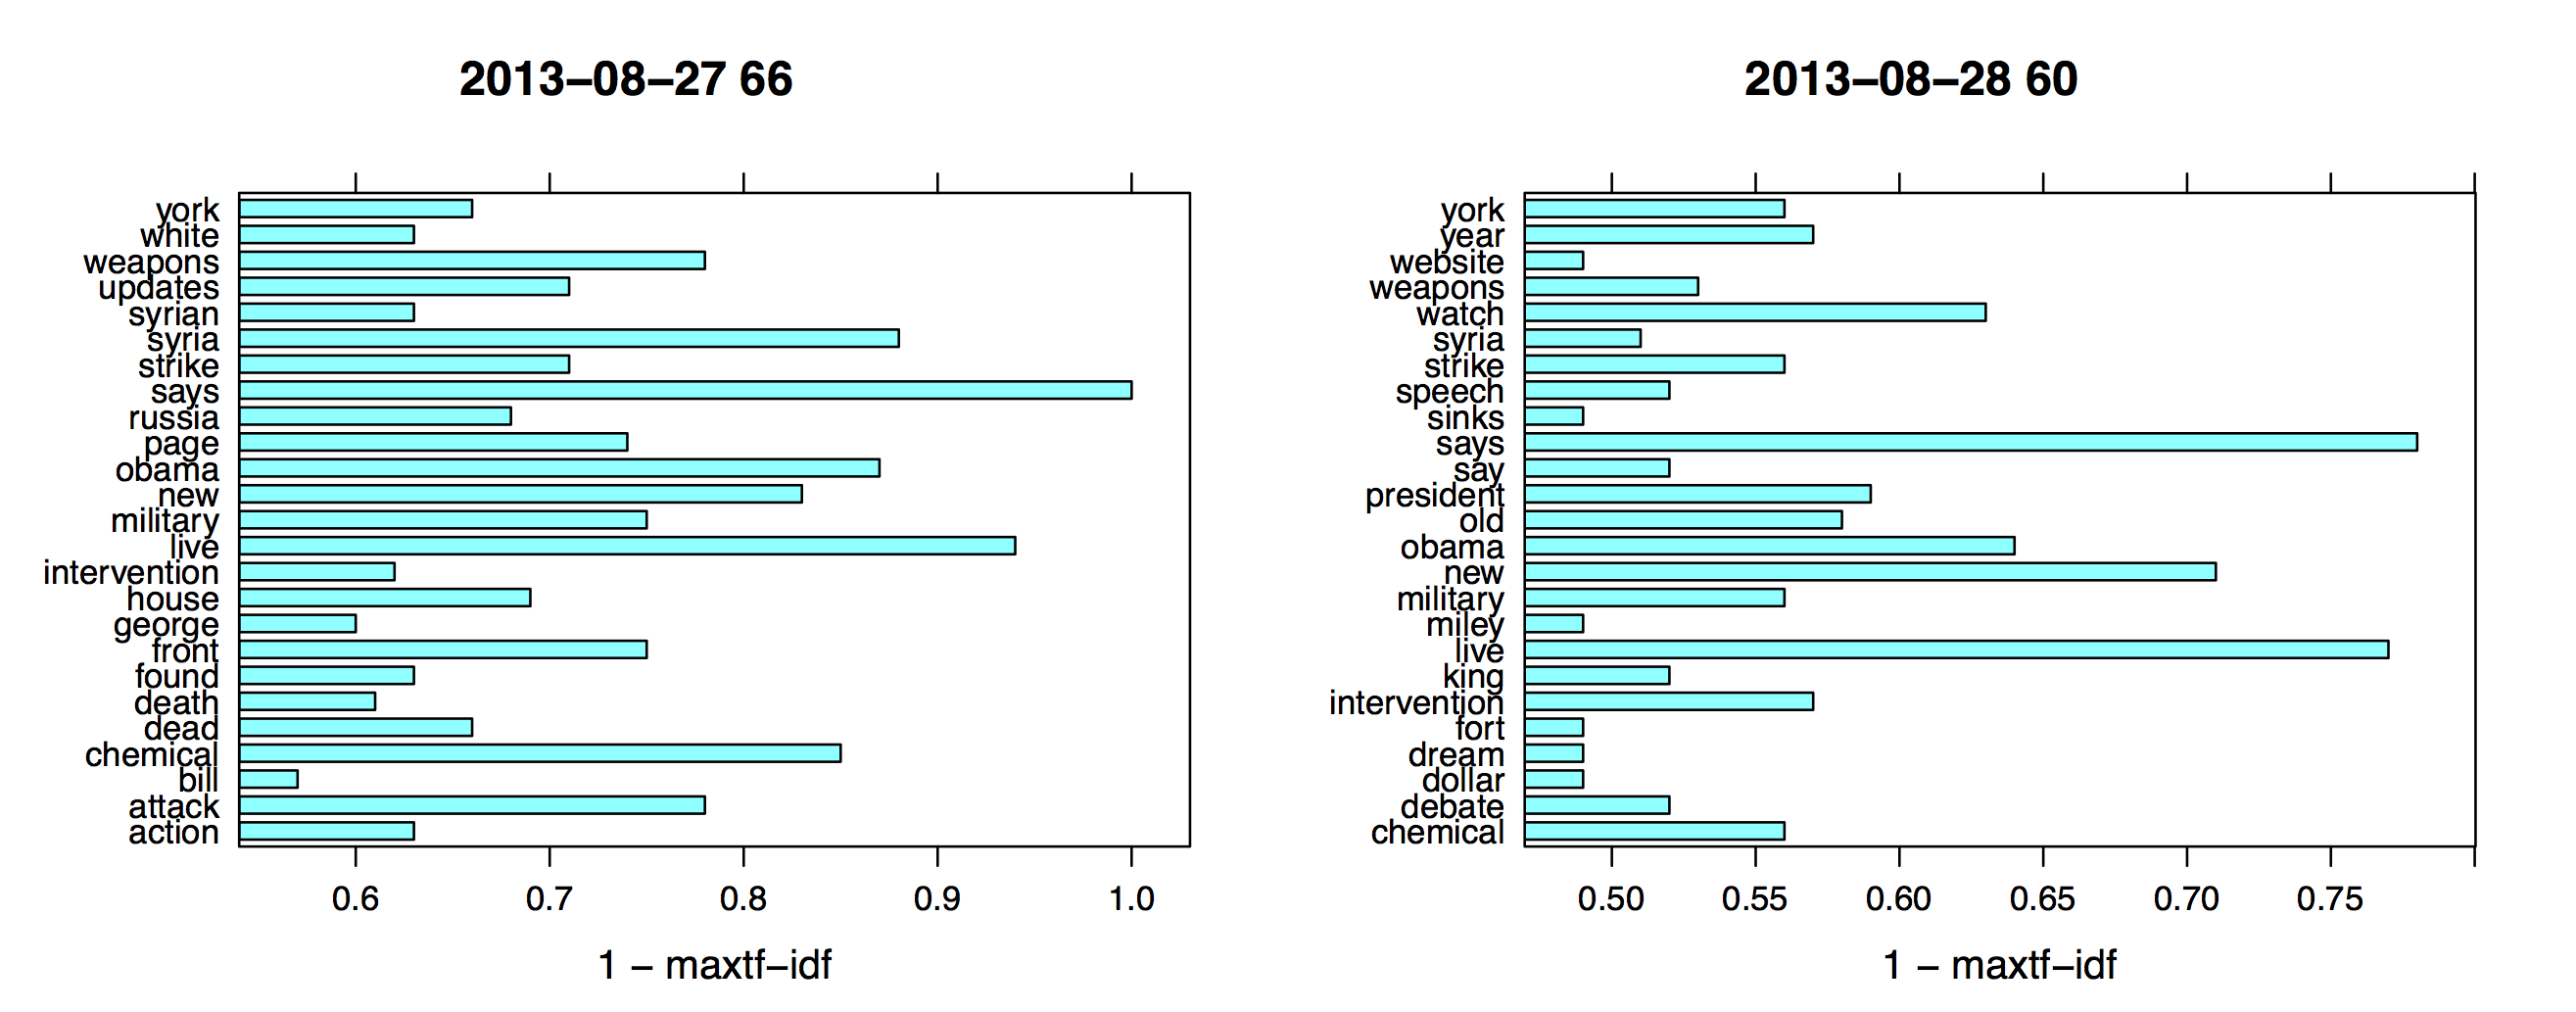
\includegraphics[width=\textwidth]{figures_SI/Plots_from_data/stopwords}
    \caption[Stopwords detection.]{\textbf{Stopwords detection.
        Normalized $1-\text{maxtf-idf}$ score for data from August
        27th (left) and August 28th (right) of 2013. The top score
        words for both plots are ``says'' and ``live''. We used the
        top score words to disconnect connected components of
        events.}}
    \label{fig:stopwords}
  \end{center}
\end{figure}


After identifying such words, the idea is to disconnect the
components connected by those words. The process is to disconnect
each component by the word with top normalized $1-\text{maxtf-idf}$
score each time until the component could not be disconnected further.
We add the top scoring words to our list of stopwords.
These words are hence ignored from the subsequent runs of the data collection methodology.
In Figure~\ref{fig:stopwords} there are two examples of this process
to identify the words.
\subsubsection{Discarding Irrelevant Tweets}
\label{subsubsec:discarding_irrelevant_tweets}

Due to the capabilities of the REST API, the tweets collected can be
older than the actual date of the event detected. For that reason,
some tweets can be very old and not relevant to the event itself. This
may lead to inaccuracies in predictions when using the early features.

This problem is illustrated in Figure~\ref{fig:duration-differences},
especially when we want to perform predictions using the first part of
the data. Note that the first 5\% of the tweets take an unusually
large portion of the duration of the entire event. This suggests that
we are collecting tweets which existed much before the event broke
out, and hence are possibly irrelevant. Once we discard the first 5\%
of tweets, we observe that each segment of the event (first 5\%, the
next 5\%, etc.) occupies roughly the same duration of the entire event.

\begin{figure}
  \centering
  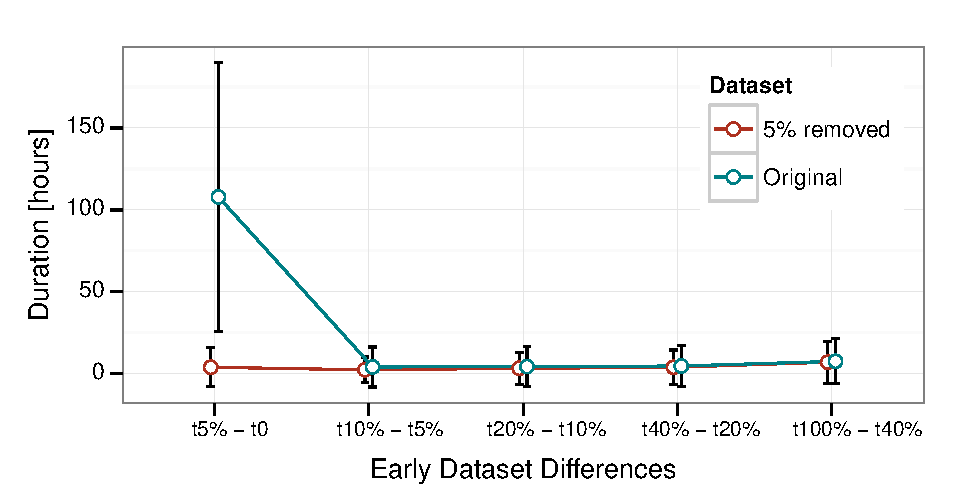
\includegraphics[width=.7\textwidth]{figures_SI/Plots_from_data/time_differences.eps}
  \caption[Duration differences of events.]{\textbf{Duration
      differences of events. The $x$-axis represents the categories of
      datasets: the first one (t5\%-t0) represents the difference of
      time between the timestamp of the oldest tweet and the newest
      tweet in the first 5\% of the tweets. The next one (t10\%-t5\%)
      corresponds to the difference between the newest tweet in the
      first 10\% and the newest tweet in the first 5\% of data, etc.
      After removing the first 5\% of data, the time differences are
      roughly the same across all datasets.
    }}\label{fig:duration-differences}

\end{figure}

\subsection{Validation of Data Collection}
We performed experiments validating that merging keywords by forming
connected components indeed produced meaningful groups of keywords
representing an event. As a baseline, we used components obtained by
merging random keyword pairs together. We evaluated how well a cluster
is formed from the set of tweets obtained from connected components,
comparing the cluster to the set of tweets obtained from random
components. Connected components are expected to merge
keyword pairs that belong to the same event, and hence would make
better clusters when compared to merging random keyword pairs. The
results are displayed in
Figure~\ref{fig:connected_components_validation}. In this figure, each
plot depicts a different metric that evaluates the quality of a
cluster. These clustering metrics are summarized in
Table~\ref{table:clustering_metrics}. For better interpretation and
visual clarity, in each of the plots, we sorted the clustering metrics
obtained via connected components. We then rearranged the clustering
metrics for the baseline according to the sorting order obtained from
connected components. (This is the reason why the blue line is
monotonically increasing.) This experiment was performed on one month
of data (there are approximately 30 data points in each plot) between
August 2013 and September 2013. We took all the keyword pairs obtained
in a day and found the connected components as in
Figure~\ref{fig:connected_components}. For random components, we
merged the keyword pairs randomly. We took precautions to make sure
that the size of the connected components and random components per
day were comparable. That is, if we had connected components of sizes
6, 6, and 5 formed from keyword pairs on particular day, we made sure
that similarly sized random components were also formed from the
keyword pairs of the same day. Also, to make sure that tweets from any
one keyword pair do not dominate the tweet set, we sampled an equal
number of tweets from each keyword pair, and the \emph{same} sample of
tweets is used to calculate the clustering metrics in both the connected
components approach and the random components approach. The random
baseline has been averaged over 3 different rounds of experimentation.

\begin{figure}
  \begin{center}
    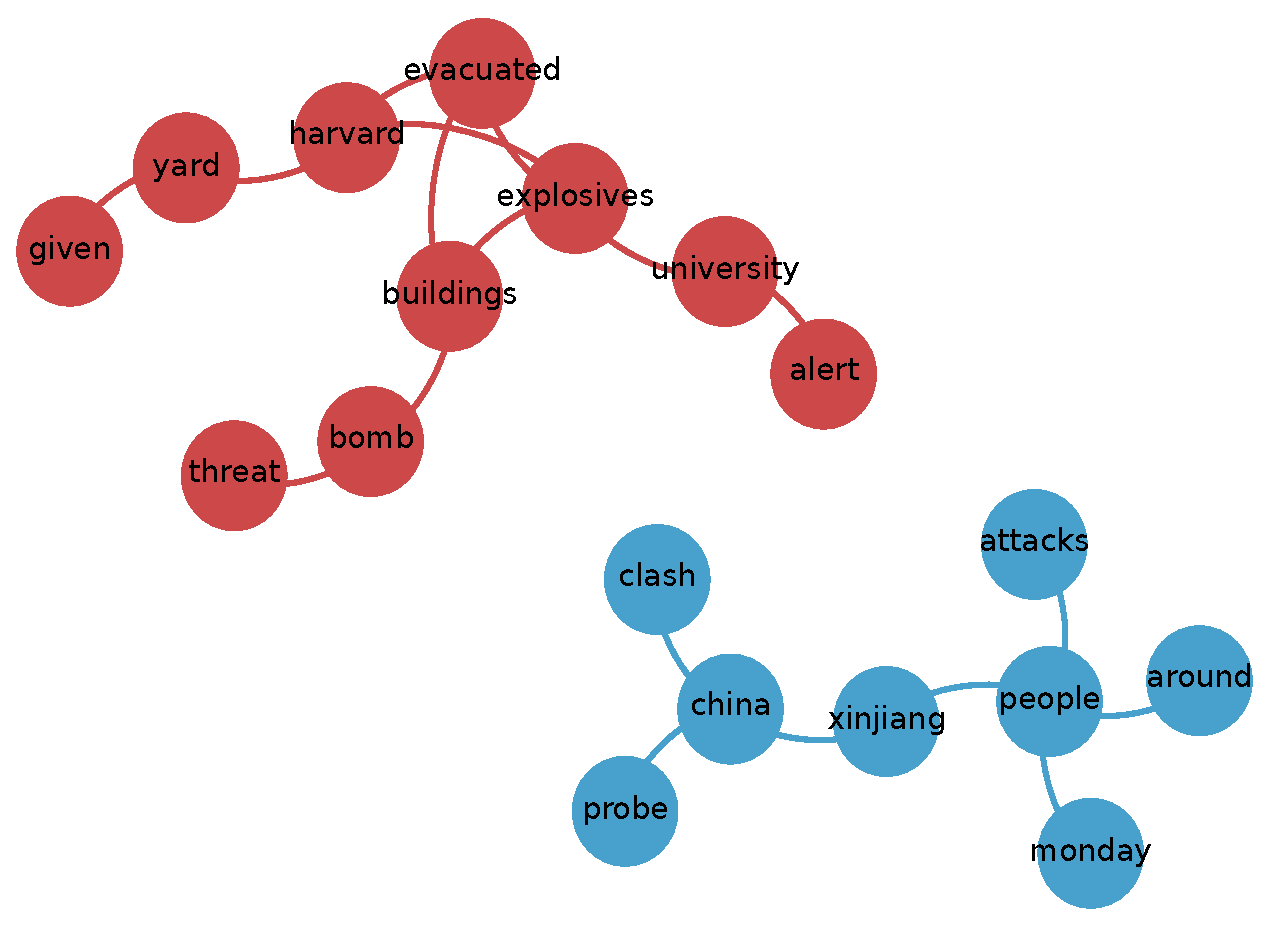
\includegraphics[width=0.7\textwidth]{figures_SI/Pictures_and_Drawings/connected_components}
    \caption{\textbf{This figure illustrates how we merge keyword
        pairs which represent the same event into larger components.
      }}
    \label{fig:connected_components}
  \end{center}
\end{figure}

\begin{figure}
  \centering
  \begin{subfigure}[b]{0.3\textwidth}
    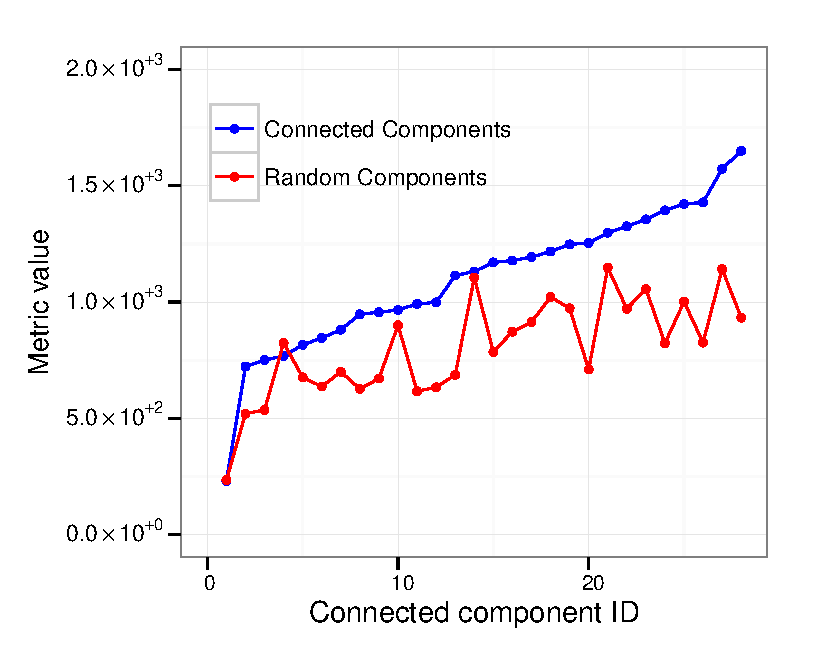
\includegraphics[width=\textwidth]{figures_SI/Plots_from_data/cc_validation/I1.eps}
    \caption{$I_1$} \label{fig:I1}
  \end{subfigure}
  \begin{subfigure}[b]{0.3\textwidth}
    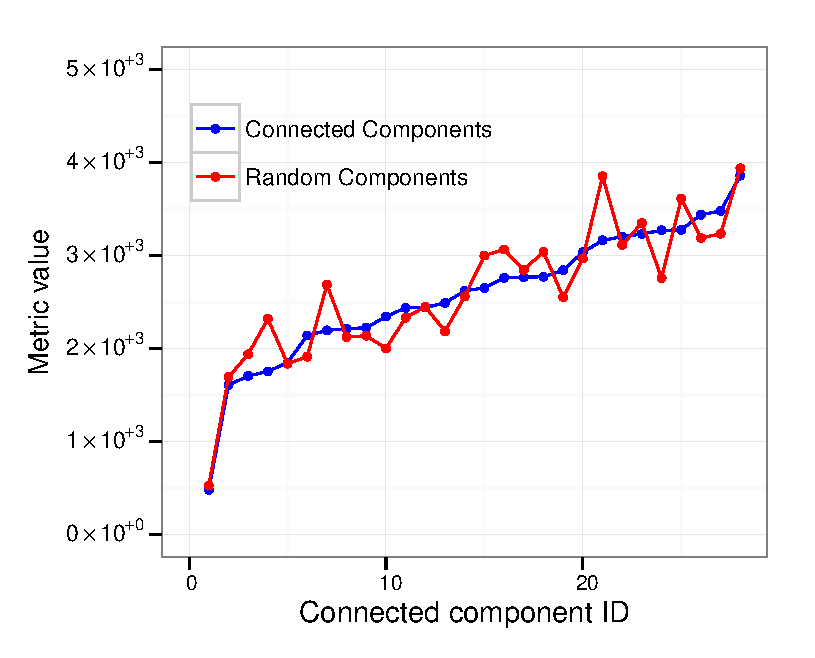
\includegraphics[width=\textwidth]{figures_SI/Plots_from_data/cc_validation/I2.eps}
    \caption{$I_2$} \label{fig:I2}
  \end{subfigure} ~ %add desired spacing
  \begin{subfigure}[b]{0.3\textwidth}
    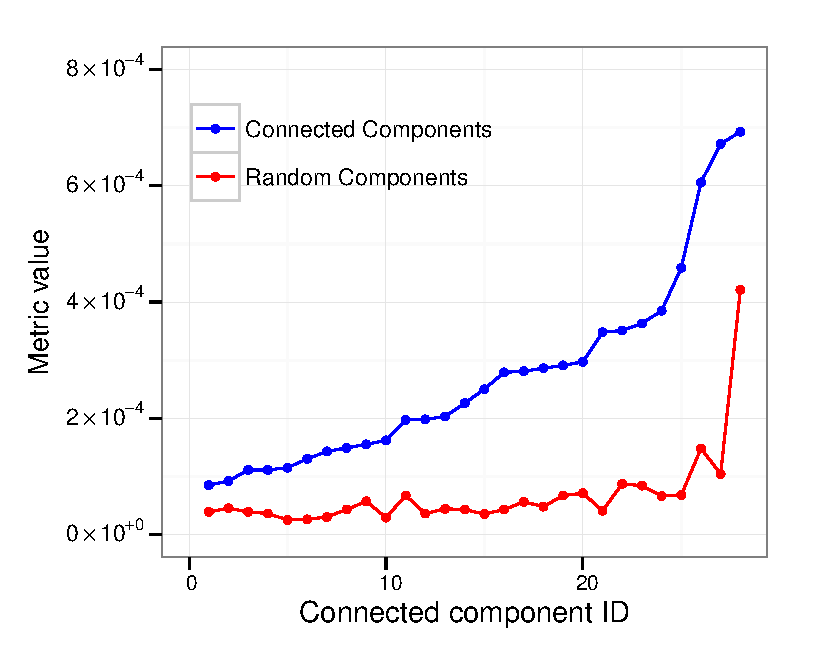
\includegraphics[width=\textwidth]{figures_SI/Plots_from_data/cc_validation/H1.eps}
    \caption{$H_1$} \label{fig:H1}
  \end{subfigure}

  \begin{subfigure}[b]{0.3\textwidth}
    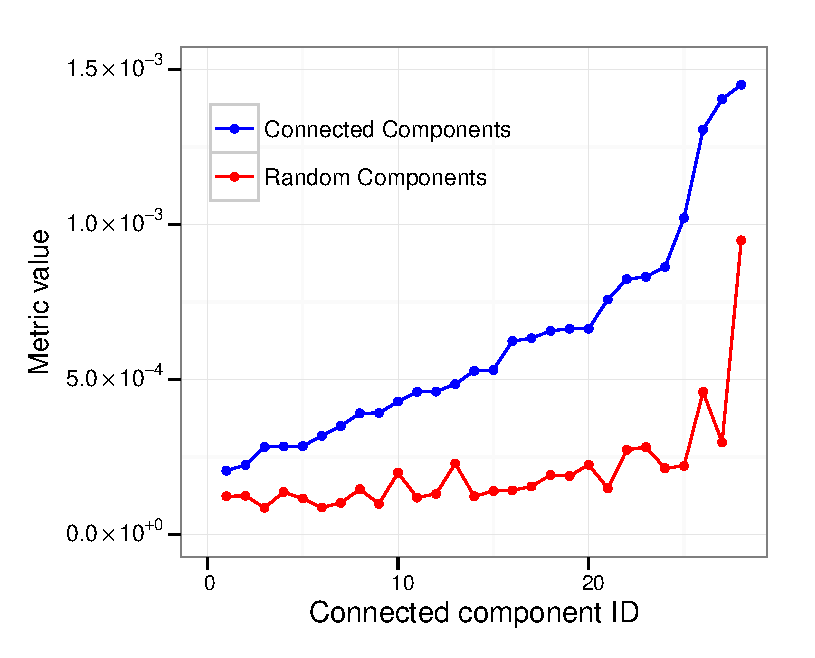
\includegraphics[width=\textwidth]{figures_SI/Plots_from_data/cc_validation/H2.eps}
    \caption{$H_2$} \label{fig:H2}
  \end{subfigure}
  \begin{subfigure}[b]{0.3\textwidth}
    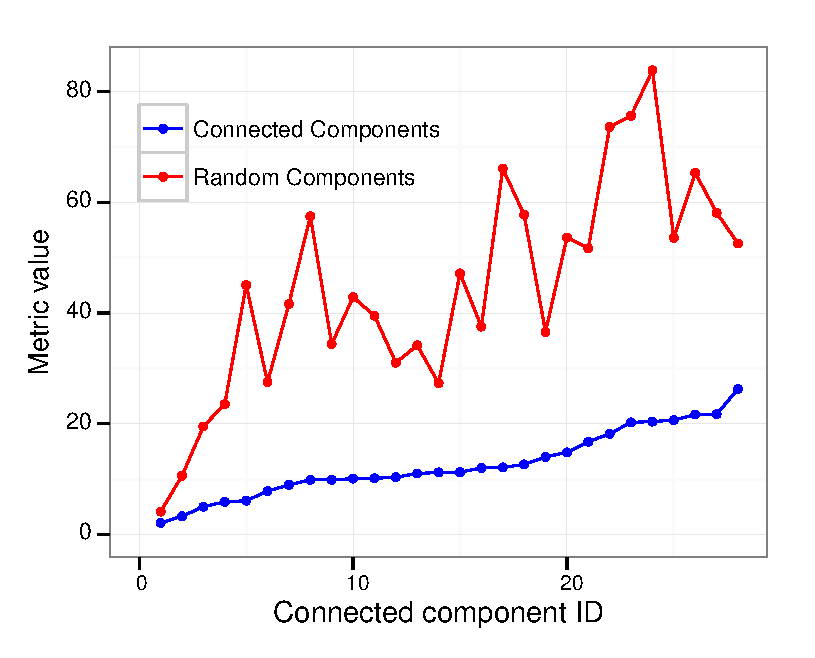
\includegraphics[width=\textwidth]{figures_SI/Plots_from_data/cc_validation/G1.eps}
    \caption{$G_1$} \label{fig:G1}
  \end{subfigure} ~ %add desired spacing
  \begin{subfigure}[b]{0.3\textwidth}
    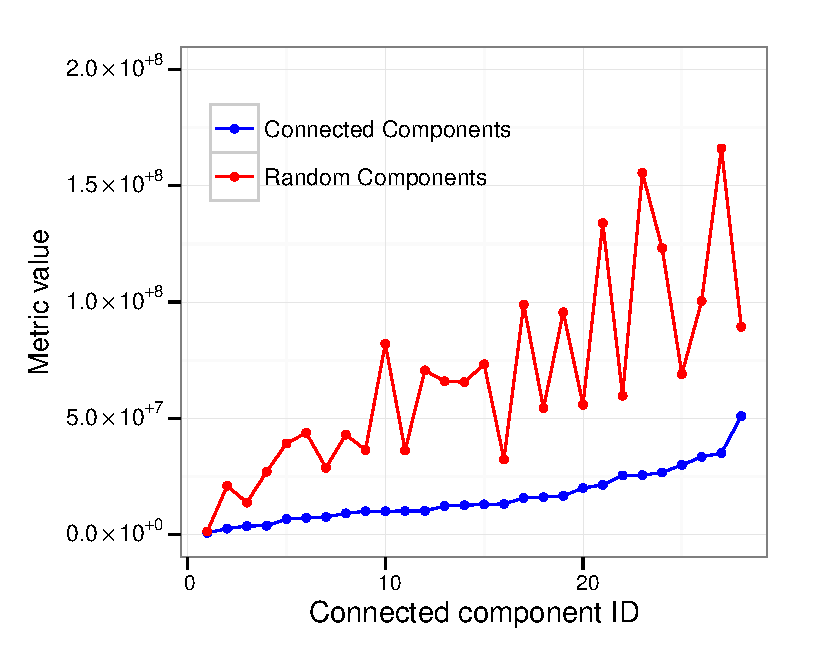
\includegraphics[width=\textwidth]{figures_SI/Plots_from_data/cc_validation/G1P.eps}
    \caption{$G'_1$} \label{fig:G1P}
  \end{subfigure}

  \caption{\textbf{Each plot in this figure compares the
          quality of the cluster of tweets obtained from connected
          components and random components. The actual metric is shown
          in Table~\ref{table:clustering_metrics}. In $I_1, I_2, H_1,
          H_2$ higher value is better. In $G_1, G_1^{'}$, lower value
          is better. For visual clarity, the values obtained from
          connected components were sorted in ascending order, hence
          the blue line is monotonically increasing. The values
          obtained were rearranged in the same order as well.}}
    \label{fig:connected_components_validation}
\end{figure}


\begin{table}
  \centering
  \begin{tabular}{ c  c  c }
    \toprule
    Name & Metric & Meaning \\
    \midrule
    $I_1$ & $\sum_{i=1}^k \frac{1}{n_i} \sum_{(u,v) \in S_i} \text{sim}(u,v)$ & Higher value is better\\
    \midrule
    $I_2$ & $\sum_{i=1}^k \sqrt{ \sum_{(u,v) \in S_i} (u,v)}$ & Higher value is better \\
    \midrule
    $E_1$ & $\sum_{i=1}^{k} n_i \frac{\sum_{v \in S_i, u \in S} \text{sim}(u,v)}{\sqrt{\sum_{(u,v) \in S_i} \text{sim}(u,v)}}$ & Lower value is better \\
    \midrule
    $G_1$ & $\sum_{i=1}^k \frac{\sum_{v \in S_i, u \in S}\text{sim}(u,v)}{\sum_{(v,u) \in S}\text{sim}(v,u)}$ & Lower value is better \\
    \midrule
    $G_1^{'}$ & $\sum_{i=1}^k n_i^2 \frac{\sum_{v \in S_i, u \in S}\text{sim}(v,u)}{\sum_{(u,v) \in S_i}\text{sim}(u,v)}$ & Lower value is better \\
    \midrule
    $H_1$ & $\frac{I_1}{E_1}$ & Higher value is better \\
    \midrule
    $H_2$ & $\frac{I_2}{E_1}$ & Higher value is better \\
    \bottomrule
  \end{tabular}
  \caption{\textbf{This table lists the clustering metrics used in Figure~\ref{fig:connected_components_validation}.}}
  \label{table:clustering_metrics}
\end{table}


\section{Event Model}
We propose a novel definition for the impact of a complex unit of
information, in this case a news event, on the Web. This definition is
motivated by the need to estimate the strength of the reaction in
terms of activity, that an event produces in Online Social Networks.
Impact should not be dependent on the size and duration of an event,
allowing us to measure both {\em global} (with large network coverage)
as well as {\em local} (with smaller network coverage) events.
Following this motivation, we present a vector model for event impact
based on the distribution of arrival interval rates between pairs of
messages. Using this representation, we can group similar events
together and identify clear separations between different types of
events.

This model is resistant to common issues that arise when estimating
network impact based on the total number of messages of an event, or
total number of shares, etc. For example, consider two events, one of
1 hour duration, and another of 100 days duration. Assume that both
events receive one hundred thousand shares in the first 20\% of their
life-span, and very little subsequent attention. If we were to
estimate their impact based on the number of shares of each event,
they might seem the same. Even when normalizing by the total duration
of each event, both events will appear equal. Nevertheless,
intuitively the event with 1 hour duration should be considered of
much higher-impact given the instancy of the reaction generated
comparatively by the network.

%%% Details %%%%
We define an event $e$, belonging to a collection of events
$\mathcal{E}$, as a tuple $(\mathcal{K}_e, \mathcal{M}_e)$, where
$\mathcal{K}_e$ is a set of \emph{keywords} and $\mathcal{M}_e$ is a
set of \emph{social media messages} or simply \emph{messages}. Both
the keywords and the messages are related to a real-world occurrence,
describing or talking about the event. The keywords are extracted in
order to succinctly describe the occurrence, and the messages are
posts from users about the event. These messages may also contain
several metadata fields like the number of times that a message has
been shared so far, or if it is part of a conversation with other
users.

We model each event $e$ based on the frequencies of the interval
arrival rates between pairs of consecutive messages in
$\mathcal{M}_e$. This model is based on a {\em vector quantization} of
these frequencies for the entire collection $\mathcal{E}$. This
approach is taken from the field of multimedia content representation,
known as {\em codebook-based representation}, used for audio and
computer-vision~\cite{ff,Vaizman}. We use this method to {\em learn}
the most representative time intervals, in order to produce a vector
for $e$. This vector represents a histogram, in which each dimension
corresponds to a learned time interval, or bin, and its value is the
percentage of consecutive pairs of messages in $\mathcal{M}_e$
contained in that bin.

To learn the representative arrival time intervals for our corpus
$\mathcal{E}$, we use the following methodology. For each $e \in
\mathcal{E}$ with messages $\mathcal{M}_e = \lbrack m_{1}^e, m_{2}^e,
\ldots m_{n}^e \rbrack$ and their corresponding time-stamps $\lbrack
t_{1}^e, t_{2}^e, \ldots t_{n}^e \rbrack$ where $t_{i} \leq t_{i+i}
\forall i \in [1,n]$, we compute all time intervals $d_{i}^e =
t_{i}^e-t_{i-1}^e$ (the value of $t_{0}$ is considered equal to
$t_{1}$ for initialization purposes). Then, the values of $d_{i}^e$
for all events in $\mathcal{E}$ are clustered to identify the {\em
  most representative} arrival time intervals present in the events.
As a cursory example to explain the process better: if all the events
that we study are extremely quick in terms of message production, then
the arrival time intervals detected by our system would probably be in
the order of microseconds. On the other hand, if our event corpus is a
mixture of different kinds of events (fast, medium, slow in message
production), then the intervals detected would vary from microseconds
to a few hours.

Once the collection bins are learned, the vector models for events is
generated. This process is summarized in
Algorithm~\ref{alg:learn_representation}.
Line~\ref{alg:line:all_time_diff} collects all of the arrival time
intervals for all the events in $\mathcal{E}$ into the vector
\textbf{f}. Line~\ref{alg:line:cluster} is a clustering algorithm
which takes the set of data points in \textbf{f} and the number of
clusters $k$ as inputs and returns the centroids of the clusters as
the output in \textbf{c}. The centroids can be thought of as the most
representative arrival time intervals over all messages. After that,
the set of arrival time intervals of each event $e$ is vector
quantized in terms of the centroids to obtain a $k$-dimensional real
valued representation of the event (Line~\ref{alg:line:vq}). This
vector representation corresponds to a histogram, where each bin, or
dimension, contains the percentage of messages with interval arrival
time within that bin (i.e., with duration between two consecutive
centroids in $c$ (Line~\ref{alg:line:cluster}).

\begin{algorithm}
  \caption{{\tt learn\_representation()}}
  \label{alg:learn_representation}
  \begin{algorithmic}[1]
    \REQUIRE Event set $\mathcal{E}$, and number of bins $k$ in the histogram.\\
    \ENSURE A representation in $\mathbb{R}^{k}$ of each event $e = (\mathcal{K}_e, \mathcal{M}_e) \in \mathcal{E}$.\\
    \STATE $\textbf{f} \leftarrow \{d_{i}^e| m_{i}^e \in
    \mathcal{M}_e, e \in \mathcal{E} \}$
    \\ \label{alg:line:all_time_diff} \STATE \textbf{c} $\leftarrow$
    {\tt cluster(}$\textbf{f}, k${\tt)} \label{alg:line:cluster}
    \FOR{$e \in \mathcal{E}$} \STATE \textbf{e} $\leftarrow$ {\tt
      vq(}$d_{i}^e, \textbf{c}$ {\tt)}\\ \label{alg:line:vq}
    \ENDFOR
  \end{algorithmic}
\end{algorithm}

\begin{figure}
  \centering
  \begin{subfigure}[b]{\textwidth}
    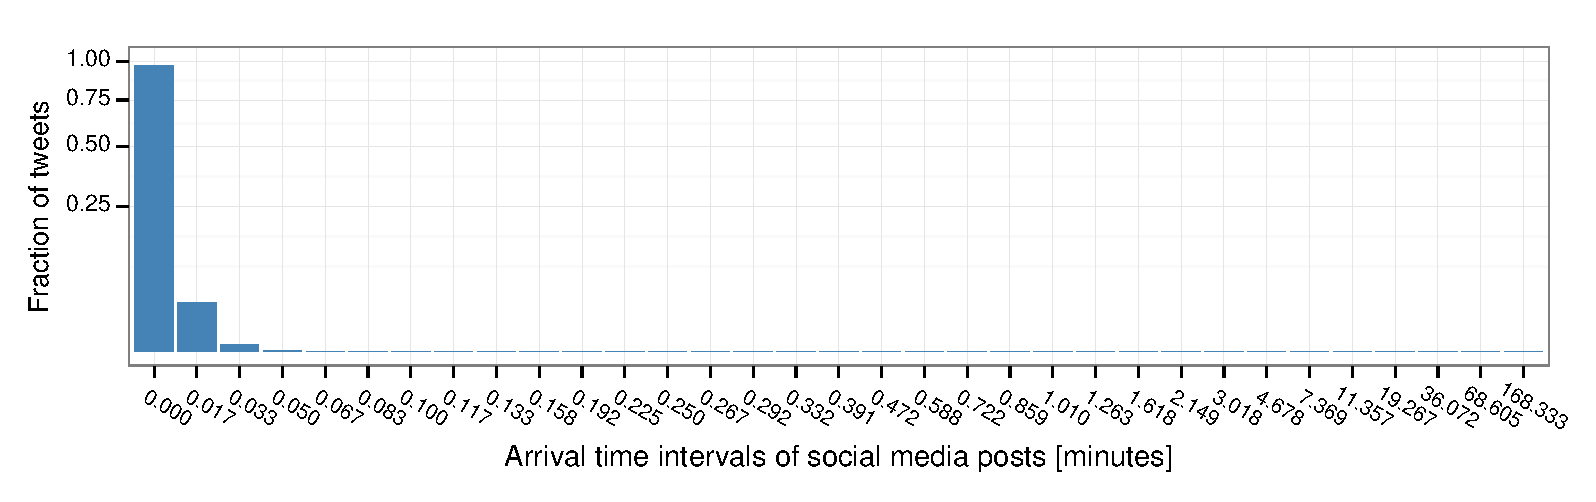
\includegraphics[width=\textwidth]{figures_SI/Plots_from_data/nelson_mandela_buzz_example}
    \caption{Death of Nelson Mandela}
  \end{subfigure}
  \begin{subfigure}[b]{\textwidth}
    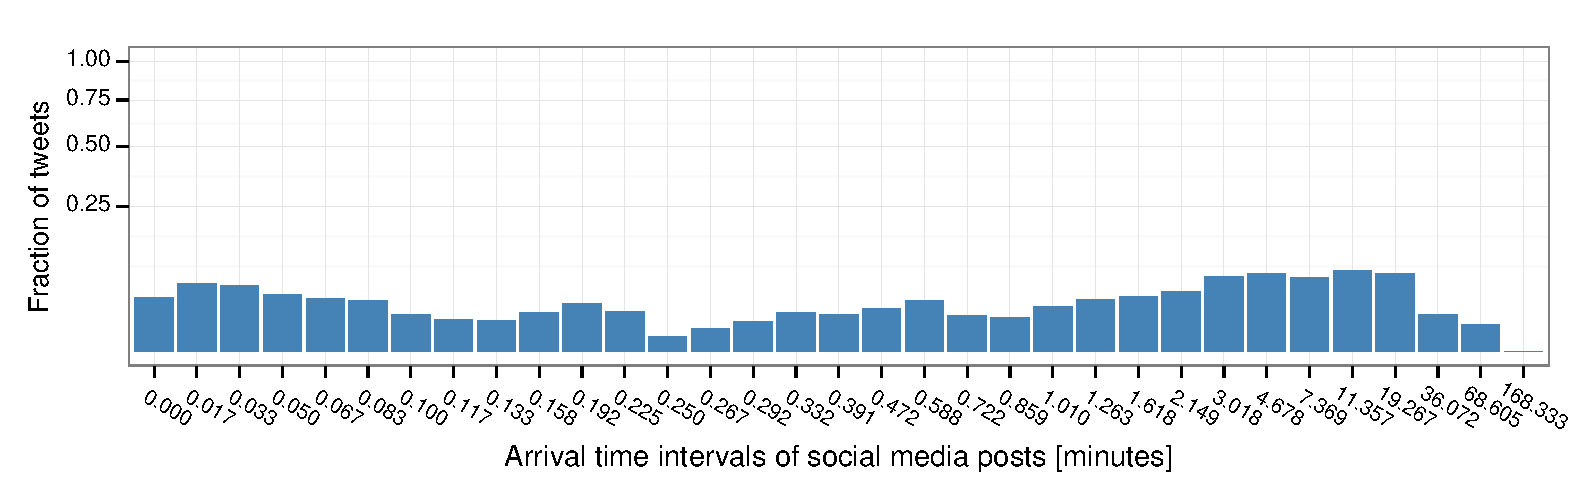
\includegraphics[width=\textwidth]{figures_SI/Plots_from_data/may_oscar_buzz_example}
    \caption{The Oscars 2014}
  \end{subfigure}
  \caption{\textbf{These figures illustrate examples of two events
      summarized by our method. The event [nelson, mandela] was
      collected on 2013-12-05 (the messages were collected from the
      Twitter social networking platform). Since there is a high
      concentration in the first bin, we conclude that the messages
      for this event occur in cascades of quick successions, almost
      instantaneously. The second event, [may, oscar], was collected
      on 2014-03-23 discussing the Oscar awards that was held a few
      weeks ago. The messages for this event are much more spread out
      in terms of how quickly they occur.}}
  \label{fig:example_buzz}
\end{figure}

Figure~\ref{fig:example_buzz} illustrates two events using the
histograms produced for their impact-based vector models created from
their arrival time intervals. The top figure corresponds to the event
\{nelson, mandela\} and was collected on December 5, 2013 soon after
the death of Nelson
Mandela \cite{nelson_mandela_dead}.
%\footnote{\url{https://en.wikipedia.org/wiki/Death_of_Nelson_Mandela}
%  (Accessed: August 25, 2015)}. 
Note that the learned bins vary from
$0$ minutes to $68$ minutes. Since there is a high concentration in
the first bin, it can be concluded that the messages for this event
appeared in instantaneous cascades of messages. For the bottom figure,
the event \{may, oscar\} was collected on March 23, 2014 discussing
the Oscars ceremony that was held a few weeks ago from that time. The
message arrival rate for this event was much more spread out.

Using the proposed impact-based representation for events, it is
possible to identify groups of similar events according to the
intensity of the overall reaction to the event. In particular,
clustering of these event vectors allows us to identify groups of
events with similar distributions of their interval arrival rates.
Intuitively, these groups of events can be sorted according to their
concentration of messages in the first bins, in order to identify
high-impact events. This procedure is independent of the volume and
duration of each event.
\section{High-impact vs low-impact: what is the difference?}
\label{sec:diff}

\begin{figure}
  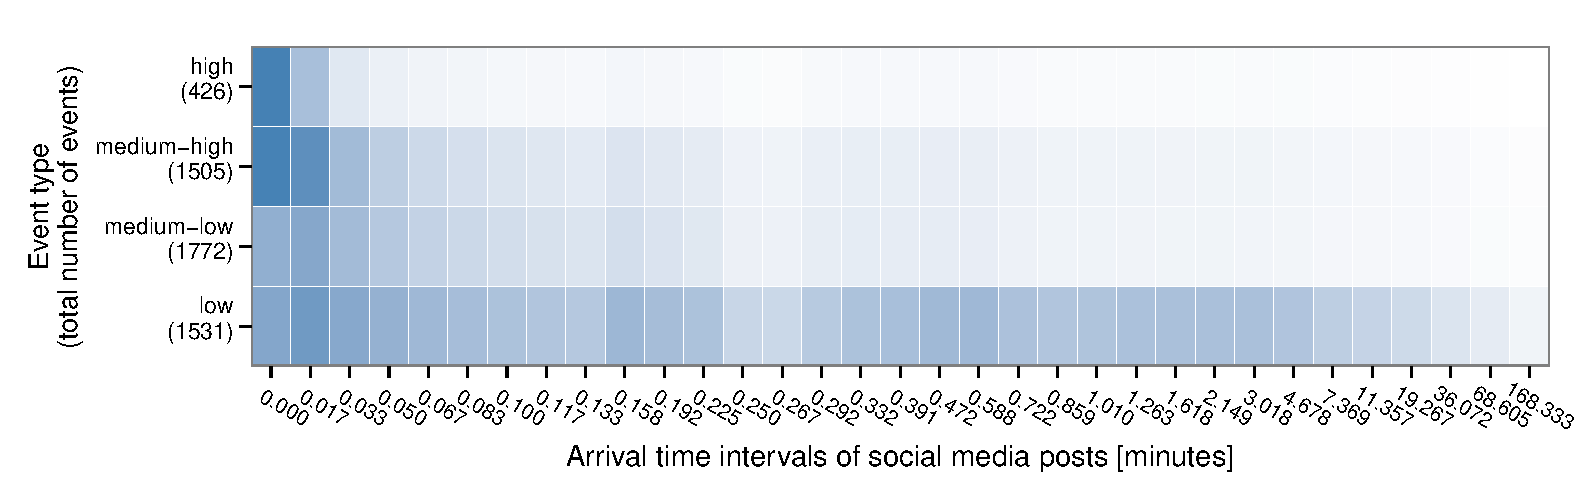
\includegraphics[width=\textwidth]{figures_SI/Plots_from_data/heatmap_summarized}
  \caption{\textbf{All the events were clustered into groups of events
      based on their message arrival rates representation. Each row in
      the figure is the average representation of all events in that
      cluster. A darker cell represents a higher value.}}
  \label{fig:low_buzz_high_buzz}
\end{figure}
\begin{table}
  \centering
  {\scriptsize
    \begin{tabular*}{1\linewidth}{p{5cm}p{5cm}}
      \hline
      Event & Sample Tweets \\
      \hline
      \pbox{20cm}{\textbf{Description:}\\ Death of American\\actor Paul Walker. \vspace{.1cm}\\
        \textbf{Keywords:}\\ {[}walker, paul{]}\vspace{.1cm}\\
        \textbf{Date:}\\ 2013-12-04}
      & \pbox{20cm}{
        @\_PaulWaIker: Every Paul Walker And Fast And Furious Fan Gotta Read This\\..GENIUS..JUST GENIUS! http://t.co/vIUZBOebvg\vspace{.1cm}\\
        @GossipCop: Paul Walkers Daughter Meadow Did NOT Witness His Death;\\ Teenage Girl Victim of Hoaxes and False Rumors http://t.co/BPyXkv8RLB\vspace{.1cm}\\
        @GAFollowers: Many of Paul Walker's Fast 7 scenes remain to be shot.\\ A final decision on whether to keep the movie as is or starting over could come soon.\vspace{.1cm}\\
        @TeamBoosieBoo: Rest in peace Paul Walker  RETWEET To Show Respect
      }
      \\
     \hline
      \pbox{20cm}{\textbf{Description:}\\ Death of South African\\ politician Nelson Mandela. \vspace{.1cm}\\
        \textbf{Keywords:}\\ {[}nelson, mandela{]}\vspace{.1cm}\\
        \textbf{Date:}\\ 2013-12-05}
      & \pbox{20cm}{
        @DaniellePeazer: RIP Nelson Mandela.....what a truly phenomenal and inspirational man xx\vspace{.1cm}\\
        @iansomerhalder: Im in tears.The world has lost one of its greatest shepherds of peace.\\Thank you Mr.Mandela for the love you radiated. http://t.co/u39MVVEKe8\vspace{.1cm}\\
        @FootballFunnys: This is so true. RIP Nelson Mandela. http://t.co/vF9xri8LdP\vspace{.1cm}\\
        @David\_Cameron: I've spoken to the Speaker and there will be statements and tributes \\to Nelson Mandela in the House on Monday.} \\
      \hline
      \pbox{20cm}{\textbf{Description:}\\ Soccer player Luis Suarez\\ bites another player in\\ 2014 FIFA World Cup. \vspace{.1cm}\\
        \textbf{Keywords:}\\ {[}fifa, world, cup, suarez,\\ luis, biting, soccer, bite{]}\vspace{.1cm}\\
        \textbf{Date:}\\ 2014-06-25}
      & \pbox{20cm}{
        @M\_arioBalotelli: CLEAR ANGLE of the Suarez bite!!  https://t.co/bI08YsZWSE\vspace{.1cm}\\
        @fifamedia: Disciplinary proceedings opened against Uruguay's Luis Suarez\\ http://t.co/w6mRNuSGZt\vspace{.1cm}\\
        @DeadlineDayLive: Luis Suarez will sign a 5-year contract at Barcelona and he'll wear \\the no. 9 shirt. (Source: http://t.co/6uRIUwjsGN) http://t.co/FxyOf9ERVr\vspace{.1cm}\\
        @GeniusFootball: BREAKING: FIFA have caught Suarez leaving the stadium?\\ http://t.co/vsQQCVV1GQ} \\
      \hline
    \end{tabular*}
  }
  \caption{\textbf{Examples of high-impact news events. The events
      shown were taken from the ``high'' category according to Figure~\ref{fig:low_buzz_high_buzz}}.}
  \label{table:high-impact-sample}
\end{table}

\begin{table}
  \centering
  {\scriptsize
    \begin{tabular*}{1\linewidth}{p{5cm}p{5cm}}
      \hline
      Event & Sample Tweets \\
      \midrule
      \pbox{20cm}{\textbf{Description:}\\US Government refuses\\ Germany to grant answers\\ or access to NSA records. \vspace{.1cm}\\
        \textbf{Keywords:}\\ {[}nsa, merkel{]}\vspace{.1cm}\\
        \textbf{Date:}\\ 2014-04-10}
      & \pbox{20cm}{
        @guardiannews: Angela Merkel denied access to her NSA file http://t.co/FLQc0zSjYJ\vspace{.1cm}\\
        @mog7546: \#GERMANY's \#Merkel says \#OBAMA's \#US assurances on \#NSA spying\\ "INSUFFICIENT" - Reuters India http://t.co/D2L52CP9YZ\vspace{.1cm}\\
        @GermanyForum: Merkel denied access to own NSA file http://t.co/e6vKCOkbXA\vspace{.1cm}\\
        @kgosztola: US ignores request from German Chancellor Angela Merkel to look at NSA file:\\ http://t.co/HFTMMZBu5W
      }
      \\
      \hline
      \pbox{20cm}{\textbf{Description:}\\75 scientists exposed\\ to anthrax. \vspace{.1cm}\\
        \textbf{Keywords:}\\ {[}may, anthrax, \\exposed, scientists{]}\vspace{.1cm}\\
        \textbf{Date:}\\ 2014-06-19}
      & \pbox{20cm}{
        @CBSEveningNews: .@CDCgov confirms 75 staff members are being monitored or provided\\ antibiotics because they may have been unintentionally exposed to anthrax\vspace{.1cm}\\
        @pettybooshwah: Atlanta CDC lab fails to follow procedure to kill anthrax,\\ ships it downstream. 75 scientists now on Cipro \&; edgy. http://t.co/TrJ9qXXzW\vspace{.1cm}\\
        @ABCWorldNews: NOW: CDC announces a breach that may have exposed workers to\\ live anthrax - What went wrong? @DrRichardBesser with details.\vspace{.1cm}\\
        @AJEnglish: Dozens of US scientists 'exposed to anthrax' http://t.co/ThGPmX4k71
      }
      \\
      \hline
      \pbox{20cm}{\textbf{Description:}\\Surveying the damages of \\ recent tornado in Canada. \vspace{.1cm}\\
        \textbf{Keywords:}\\ {[}canada, tornado{]}\vspace{.1cm}\\
        \textbf{Date:}\\ 2014-06-21}
      & \pbox{20cm}{
        @Kathleen\_Wynne: Visited \#Angus today to survey the damage. Thankfully no fatalities\\ or major injuries from recent tornado. http://t.co/xRQyRWg5Vw\vspace{.1cm}\\
        @SunNewsNetwork: PHOTOS \& VIDEO: Hundreds displaced after tornado hits Ontario town,\\ destroying homes http://t.co/L38rG6N1a6\vspace{.1cm}\\
        @CBCToronto: Kathleen Wynne is speaking at site of tornado damage in Angus, Ont. now.\\ Watch live here: http://t.co/EDKNUiZo0X \#cbcto\vspace{.1cm}\\
        @InsuranceBureau: @CTVBarrieNews: Insurance Bureau of Canada is setting up a mobile unit\\ in \#Angus today to help residents affected by \#Tornado}
      \\
      \hline
    \end{tabular*}
  }
  \caption{\textbf{Examples of non-high-impact news events. The events
      shown were taken from the ``low'' category according to Figure~\ref{fig:low_buzz_high_buzz}}.}
  \label{table:low-impact-sample}
\end{table}
%\input{events_examples.tex}

After collecting a dataset of events from Twitter, we use
Algorithm~\ref{alg:learn_representation} to learn the representation
for each event. We use \texttt{kmeans} as the clustering method for
Algorithm~\ref{alg:learn_representation} (Line 2). Based on the
obtained representations, the events are clustered and we obtain 20
groups of similar events in terms of their arrival rates.
Figure~\ref{fig:low_buzz_high_buzz} shows the average event
representation in different cluster groups, each group consisting of
five consecutive clusters, sorted by their average value in the first
dimension of the event representation. A darker color implies higher
value in that cell. As we move from the top to the bottom, there is a
gradual shift in the arrival rate of tweets.

\begin{figure}
  \centering
  \begin{subfigure}[b]{0.5\textwidth}
    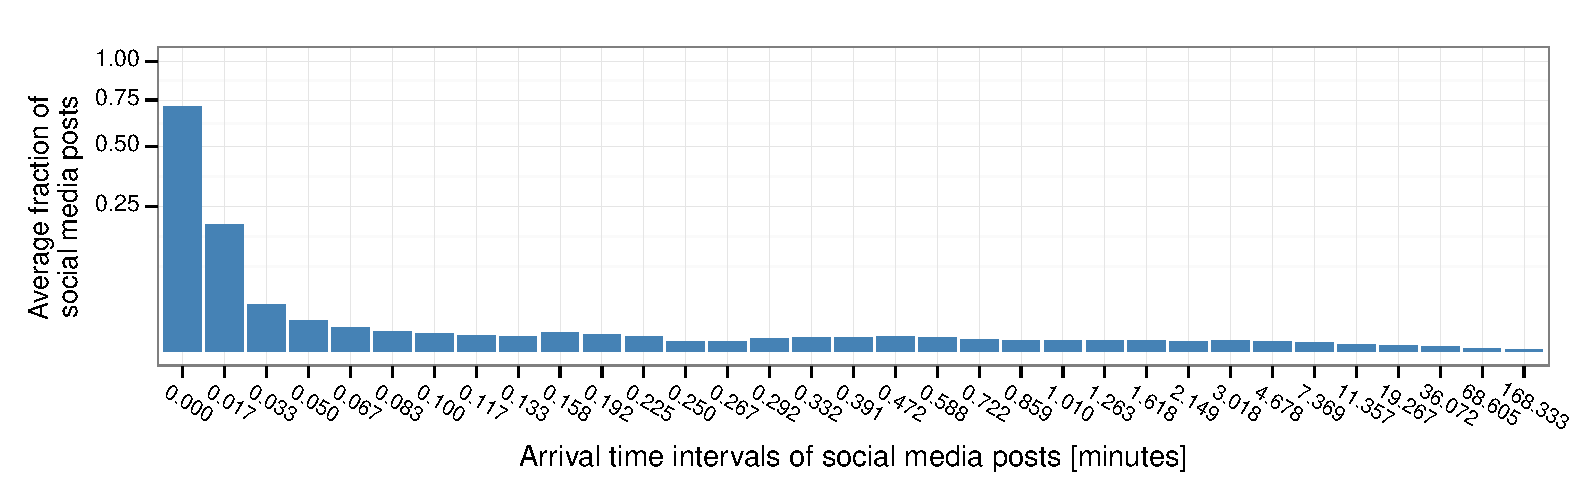
\includegraphics[width=\textwidth]{figures_SI/Plots_from_data/avg_hist_3_7}
    \caption{High impact events}
    \label{fig:highest}
  \end{subfigure}%
  ~
  \begin{subfigure}[b]{0.5\textwidth}
    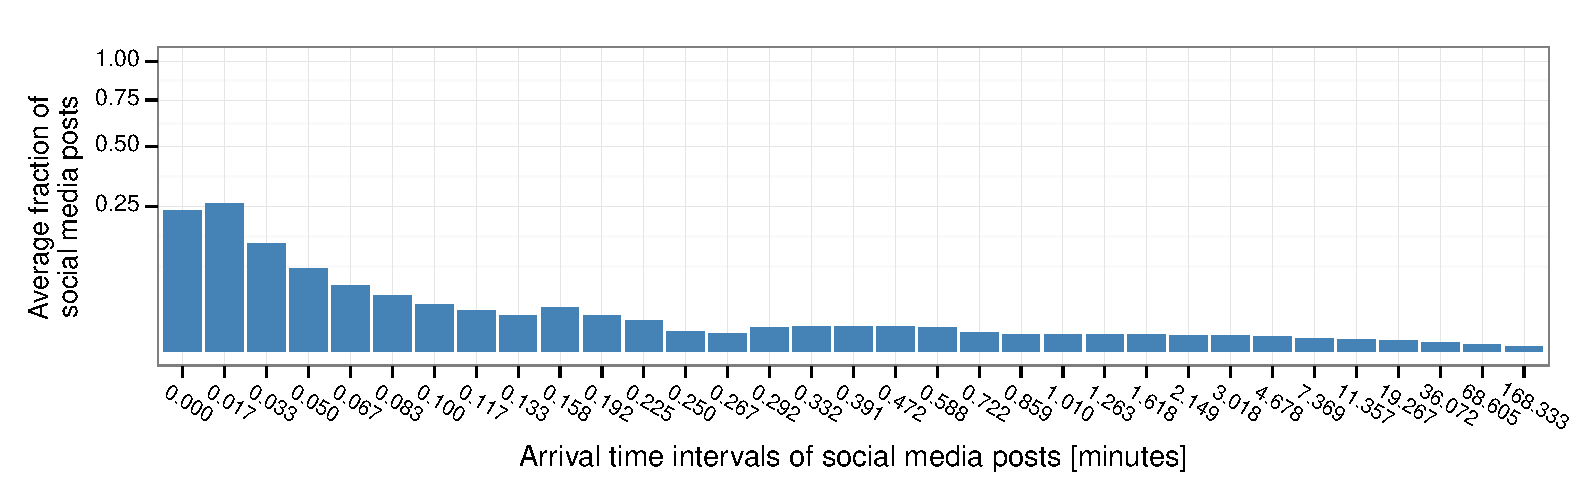
\includegraphics[width=\textwidth]{figures_SI/Plots_from_data/avg_hist_19_16}
    \caption{Medium-high impact events}
    \label{fig:high}
  \end{subfigure}%
  ~

  \begin{subfigure}[b]{0.5\textwidth}
    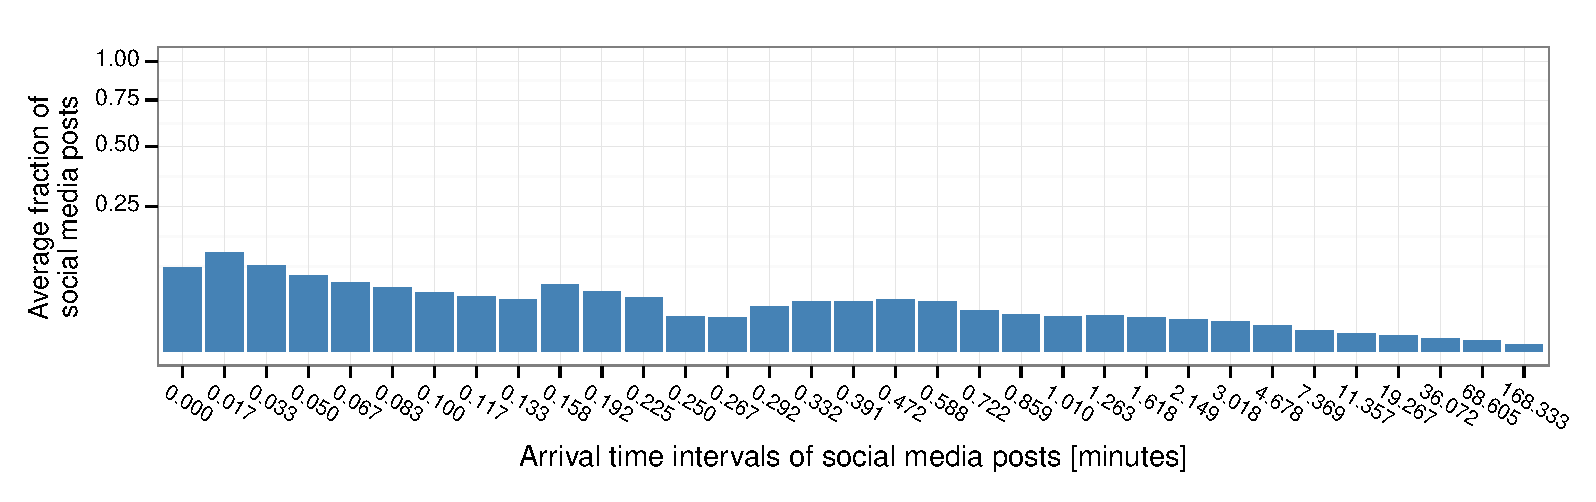
\includegraphics[width=\textwidth]{figures_SI/Plots_from_data/avg_hist_11_9}
    \caption{Medium-low impact events}
    \label{fig:med}
  \end{subfigure}%
  ~
  \begin{subfigure}[b]{0.5\textwidth}
    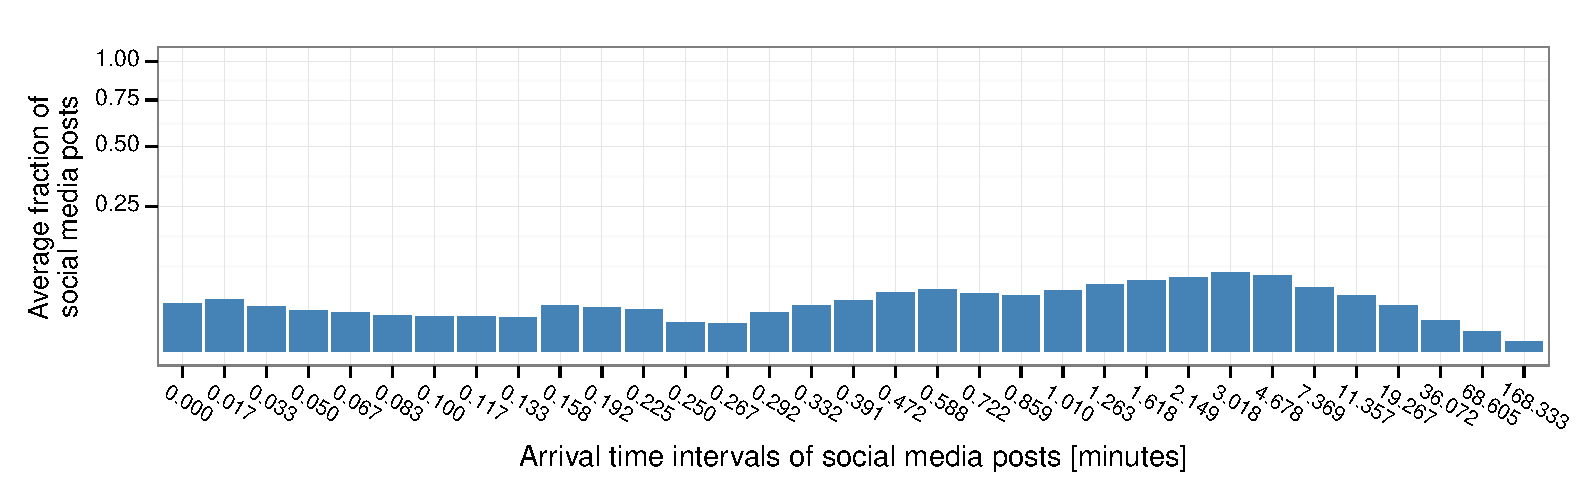
\includegraphics[width=\textwidth]{figures_SI/Plots_from_data/avg_hist_0_1}
    \caption{Low impact events}
    \label{fig:low}
  \end{subfigure}%
  ~
  \caption{\textbf{Average histograms of impact from selected clusters
      of events. The bar at each bin corresponds to the average
      fraction of messages for those event clusters (in square root
      scale). Figure~\ref{fig:highest} shows the histogram of the top
      high-impact events in our dataset. Figure~\ref{fig:high} shows
      two other clusters in descending ranking of impact. The same for
      Figure~\ref{fig:med} and Figure~\ref{fig:low}, where the last
      one shows the histogram of the lowest
      ranking.}}\label{fig:histograms}
\end{figure}

%\begin{table}
%  \centering
%  {\small
%    \begin{tabular}{cc}
%      \toprule
%      Cluster Numbers &  Fraction of all events occupied by clusters\\
%      \midrule
%      $3,7$ &  $8.14$\% of all events\\
%      % \midrule
%      $3,7,10$ & $15.11$\% of all events \\
%      % \midrule
%      $3,7,10,12$ & $24$\% of all events \\
%      % \midrule
%      $3,7,10,12,14$ & $33$\% of all events \\
%      \bottomrule
%    \end{tabular}
%  }
%  \caption{\textbf{This table shows what percentage of data some subsets of the clusters
%      occupy.  We use these sets of clusters to study how the events in these categories
%      differ from the rest.}}
%  \label{tab:threshold}
%\end{table}

\begin{table}
  \centering
  {\small
    \begin{tabular}{cc}
      \toprule
      Event clusters considered &  Fraction of all events occupied by clusters\\
      \midrule
      top-2 clusters &  $8.14$\% of all events\\
      % \midrule
      top-3 clusters & $15.11$\% of all events \\
      % \midrule
      top-4 clusters & $24$\% of all events \\
      % \midrule
      top-5 clusters & $33$\% of all events \\
      \bottomrule
    \end{tabular}
  }
  \caption{\textbf{This table shows what percentage of data some
      subsets of clusters occupy. The clusters corresponds to the ones
      obtained according to Section~\ref{sec:diff}. The first clusters
      are considered to be of higher impact than the following ones,
      according to the ordering of Figure~\ref{fig:low_buzz_high_buzz}.
      We use these sets of clusters to study how the events in these
      categories differ from the rest.}} 
  \label{tab:threshold}
\end{table}


Figure~\ref{fig:histograms} also illustrates the differences between
the different types of events (similar to
Figure~\ref{fig:low_buzz_high_buzz}, but in a histogram format). To
show some examples, we sampled some events from clusters of
Figure~\ref{fig:highest} and~\ref{fig:low} and summarize them
in Tables~\ref{table:high-impact-sample}
and~\ref{table:low-impact-sample}.


%To show differences between different event groups,
%Figure~\ref{fig:histograms} shows four pairs of clusters, in
%decreasing order of impact, being Figure~\ref{fig:highest} the top two
%clusters considered, and Figure~\ref{fig:low} the bottom two clusters.
%Tables~\ref{table:high-impact-sample} and
%\ref{table:low-impact-sample} show some examples of events sampled
%from the clusters.

We want to discover semantic characteristics of high-impact events
that differentiate them from the rest. As explained earlier, Twitter
users can perform several actions like `favorite' a tweet, or
`retweet' a tweet. These actions can be perceived as some form of
social signaling by the users. For example, if an event tends to have
a high retweeting rate, it possibly means that the general trend in
the network is to spread information about the occurrence of the
event. These are the kind of features that we want to analyze to see
how high-impact events are different from others.

Based on Figures~\ref{fig:example_buzz}
and~\ref{fig:low_buzz_high_buzz}, it is clear that some groups of
events have a very unique behavior in terms of the tweet arrival
rates. We consider thresholds as in Table~\ref{tab:threshold} and
separate approximately the top 8\%, 15\%, 24\% and 33\% of events. We
study how higher impact events are different from others, and analyze
at what stage of an event's evolution do the differences begin to kick
in. We consider the top 8\% of the events (refer to
Figure~\ref{fig:highest}) to be high-impact, and perform two tailed
t-tests for each of the considered features. In general, high-impact
events have several features which markedly differentiate them from
other events. By grouping appropriate features together, we interpret
these differences as some semantically meaningful behavior.

\subsection{Information Forwarding Characteristics}
\label{subsec:info_forwarding}
We found that the high-impact events possess more information
forwarding characteristics than other events. We present four features
which support this argument. The features, their description and their
values are listed in Table~\ref{tab:information_forwarding}.


The \texttt{retweet\_count} is generally higher for high-impact
events. This feature is the fraction of retweets present in the event,
log-normalized by the total amount of tweets in the event. A higher
value suggests that people have a greater tendency to spread the
occurrence of these events. According the separation we made,
high-impact events had tweets arriving at a much faster rate than
others. It makes sense that this fast arrival rate is due to people
quickly choosing to retweet on the event, as opposed to writing their
own original phrasing of the event itself.

The \texttt{tweets\_retweeted} is lower for high-impact events than
for the rest. This feature is the number of tweets which have been
retweeted, log-normalized by the total number of tweets in the event.
This suggests that the high amount of retweets for the high-impact
events actually originates from fewer tweets. Intuitively it makes
sense that for high-impact events, fewer tweets become popular and are
retweeted several times.

The \texttt{retweets\_most\_retweeted} is much higher for high-impact
events than for low impact events, suggesting that the most popular
tweet indeed becomes very popular when the event is of high-impact.
This feature is the total amount of retweets of the tweet that has
been retweeted most.

Figure~\ref{fig:info_forward_hypothesis} comprehensively illustrates
the behavior for the information forwarding features through all the
phases of both high-impact and non-high impact events. The
\texttt{retweet\_count} has an upward trend as the event progresses.
The upward trend shows that the retweet count grows over time. This is
fairly obvious since we are cumulatively counting the retweets as the
event progresses, and it has to be non-decreasing over time. It is
however interesting that the \emph{rate} at which this curve grows is
constant; that is, the second derivative seems to be approximately a
flatline. The feature \texttt{retweets\_most\_retweeted} also has an
upward trend as the event progresses. Specifically, this upward trend
seems to have a non-negative second derivative. This suggests that the
most retweeted tweet actually gets the bulk of its retweets as time
progresses. Putting together the two features, \texttt{retweet\_count}
and \texttt{retweets\_most\_retweeted}, we may expect the sharper
upward trend in \texttt{retweets\_most\_retweeted} to show in
\texttt{retweet\_count}, but it does not seem to. This could possibly
be because the number of retweets that the most retweeted tweet
receives is indeed a small fraction of the total number of retweets
for it to have a significant effect on the overall trend.

The feature \texttt{tweets\_retweeted} has a downward trend over time.
The downward trend suggests there are a few interesting tweets in the
beginning of the event (which get retweeted several times) but as the
event progresses, not many newer tweets get similar attention. If we
look at the combined behavior of \texttt{tweets\_retweeted} together
with \texttt{retweets\_most\_retweeted}, it suggests that not many
tweets get discovered for retweeting overtime. It is in the first
phase of the event that the most interesting tweets get discovered.
However, these tweets actually gain a lot of retweet counts only as
the event makes sufficient progress.

\begin{table}
  \centering
  {\scriptsize
    \begin{tabular}{llll}
      \toprule
      Feature Name &  \multicolumn{1}{l}{Description} & High-impact, Non-high-impact value & Hypothesis, $p$-value\\
      \midrule
      \texttt{retweet\_count} & \pbox{20cm}{$\log($total retweet count \\in the event divided by total\\ tweets in the event$)$} & $2.205, 1.473$ & $1$, $p = 0$ \\
      \midrule
      \texttt{tweets\_retweeted} & \pbox{20cm}{$\log($number of tweets \\retweeted divided by\\ total tweets in the event$)$} & $-1.091, -0.964$ & $1$, $p = 2.7\times10^{-5}$ \\
      \midrule
      \texttt{retweets\_most\_retweeted} & \pbox{20cm}{number of tweets of the most \\retweeted tweet} & $284.491, 40.261$ & $1$, $p = 0$ \\
      \bottomrule
    \end{tabular}
  }
  \caption{\textbf{(Refer to Section~\ref{subsec:info_forwarding}.) This table lists all the features which characterize the information forwarding aspect of an event.  In general, High-impact events tend to have higher values for information forwarding features than other events.}}
  \label{tab:information_forwarding}
\end{table}


% \begin{table}
%  \centering
%  {\small
%    \begin{tabular}{ ll }
%      \toprule
%      Feature Name &  Description \\
%      \midrule
%      \texttt{retweet\_count} & \pbox{20cm}{$\log($total retweet count in the event divided by total tweets in the event$)$}\\
%      \midrule
%      \texttt{tweets\_retweeted} & \pbox{20cm}{$\log($number of tweets retweeted divided by total tweets in the event$)$} \\
%      \midrule
%      \texttt{retweets\_most\_retweeted} & \pbox{20cm}{(number of tweets of the most retweeted tweet)}\\
%      \bottomrule
%    \end{tabular}
%  }
%  \caption{\textbf{(Refer to Section~\ref{subsec:info_forwarding}). This table lists and describes all the features associated
%      to the information forwarding aspect of an event.}}
%  \label{tab:information_forwarding_description}
%\end{table}
\begin{figure}
  \centering
  \begin{subfigure}[b]{0.45\textwidth}
    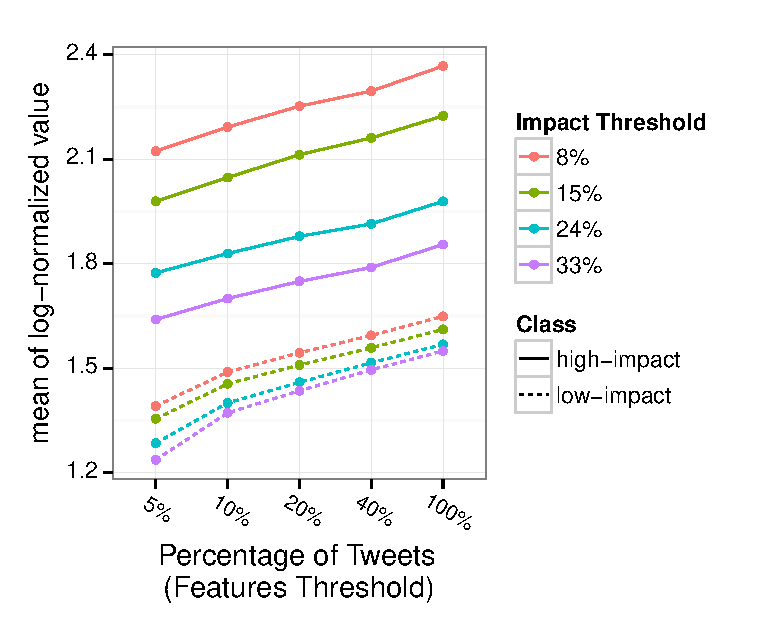
\includegraphics[width=\textwidth]{figures_SI/Plots_from_data/total_rt_count.eps}
    \caption{Retweet count.} \label{fig:feat_rt_count}
  \end{subfigure}
  ~ %add desired spacing between images, e. g. ~, \quad, \qquad,
  % \hfill etc.
  % (or a blank line to force the subfigure onto a new line)
  \begin{subfigure}[b]{0.45\textwidth}
    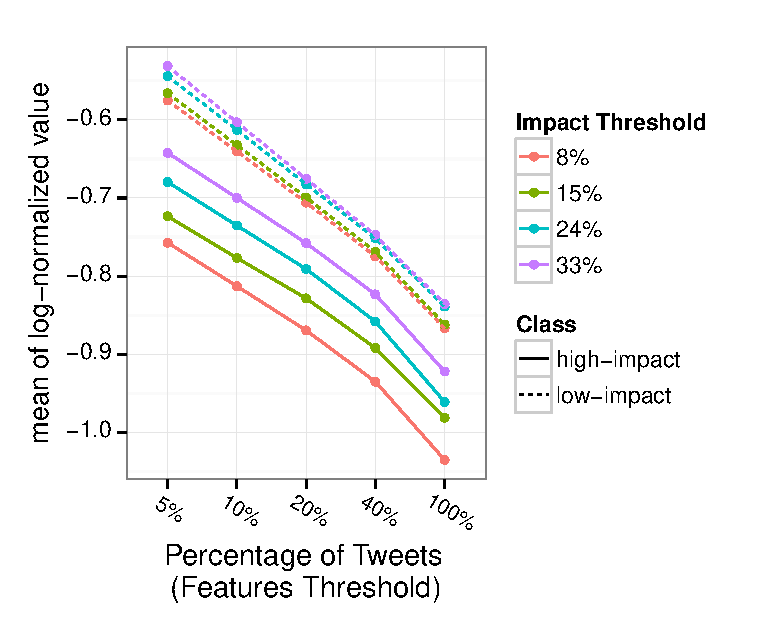
\includegraphics[width=\textwidth]{figures_SI/Plots_from_data/retweets_most_retweeted.eps}
    \caption{Retweets most retweeted.} \label{fig:feat_rt_most_rt}
  \end{subfigure} ~ %add desired spacing
  % between images, e. g. ~, \quad,
  % \qquad, \hfill etc. %(or a blank line
  % to force the subfigure onto a new
  % line)

  \begin{subfigure}[b]{0.45\textwidth}
    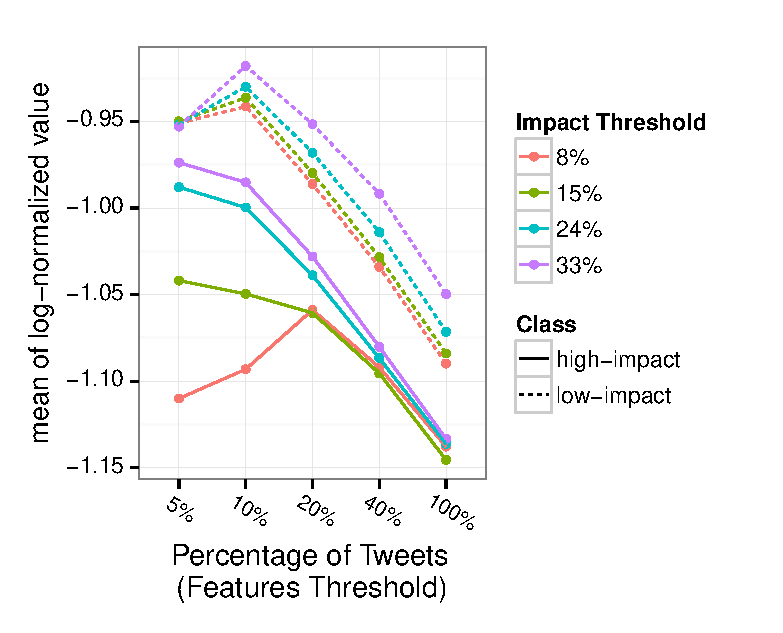
\includegraphics[width=\textwidth]{figures_SI/Plots_from_data/total_tweets_retweeted.eps}
    \caption{Total tweets retweeted.} \label{fig:feat_tweets_rt}
  \end{subfigure}
  \caption{\textbf{This figure illustrates how the features which
      explain the information forwarding characteristics differ
      between the high-impact and non-high impact events. The $x$-axis
      represents the progression of feature values as the event
      progresses. Each point on the graph represents the average value
      of the feature in all the high-impact and non-high impact events
      respectively. All solid lines represent high-impact events and
      all dashed lines represent non-high impact events. The different
      colors correspond to the results when the threshold of what is
      considered high-impact varies from the top 8\% to 33\%.
    }}\label{fig:info_forward_hypothesis}
\end{figure}

\subsection{Conversational Characteristics}
\label{subsec:conversational}
We found that high-impact events in general tend to generate more
conversation between users than low impact events. We observe this
behavior through several features. Refer to
Table~\ref{tab:conversational}.

\begin{table}
  \centering
  {\scriptsize
    \begin{tabular}{llll}
      \toprule
      Feature Name &  \multicolumn{1}{l}{Description} & High-impact, Non-high-impact value & Hypothesis, $p$-value\\
      \midrule
      \texttt{replies} & \pbox{20cm}{$\log($total replies divided by total tweets$)$} & $-1.4016, -1.6474$ & $1$, $p = 10^{-4}$ \\
      \midrule
      \texttt{norm\_replies} & \pbox{20cm}{$\log($number of replies divided by\\ total number of unique users$)$} & $-1.5796, -1.9294$ & $1$, $p = 6.7\times10^{-4}$ \\
      \midrule
      \texttt{tweets\_replied} & \pbox{20cm}{$\log($number of tweets which generated\\ replies divided by total tweets$)$} & $-1.7784, -2.0668$ & $1$, $p = 0.001$ \\
      \midrule
      \texttt{uniq\_users\_replied} & \pbox{20cm}{$\log($unique users who have written\\ a reply divided by total tweets$)$} & $-1.7524, -2.0352$ & $1$, $p = 0.001$ \\
      \bottomrule
    \end{tabular}
  }
  \caption{\textbf{(Refer to Section~\ref{subsec:conversational}.)
      This table lists all the features which characterize the conversational aspect of high-impact and non-high-impact events. Using
      these features, we argue in Section~\ref{subsec:conversational} that high-impact events tend to invoke more conversation amongst
      users than their counterparts.}}
  \label{tab:conversational}
\end{table}

The features \texttt{replies} and \texttt{norm\_replies} both count
the number of replies, but have been normalized slightly differently.
Both have a higher value for high-impact events than for low impact
events suggesting that high-impact events in general tend to spark
more conversation between the users. The \texttt{tweets\_replied}
feature counts the number of tweets which have generated replies (it
has been log-normalized by the total number of tweets in the event).
This is also higher for high-impact events than for low impact events,
indicating that high-impact events, on average have more tweets which
invoke a reply from people. The \texttt{uniq\_users\_replied} feature
counts the number of unique users who have participated in an
conversation. Again, this number is found to be higher for high-impact
events than for others, suggesting that more users tend to engage in a
conversation about events which are of high-impact. All these features
suggest that high-impact events tend to have a \emph{conversational
  characteristic} associated with them.


Figure~\ref{fig:conversational_hypothesis} comprehensively illustrates
the behavior of the conversational hypothesis of the features through
all the phases of both high-impact and non-high impact events. We
found interesting that the behavior of all these features seem to attain a
plateau at a similar value towards the end of the event. The most
remarkable differences are seen in the beginning phases of the event.
Note that for all the features, a higher value indicates a higher
conversational aspect within the event. We can infer from the plots
that, the high-impact events, from the very start have a much higher
conversational aspect. But, as the event progresses, the marginal
increase in the amount of conversation decreases and eventually
attains a plateau. On the other hand, the non-high impact events,
start with a lower conversational aspect, but pick up quickly. But
towards the end of the event, they plateau as well.

This behavior perhaps suggests that there is only a fixed amount of
``conversation" any event can evoke. It is the initial response to
these events that seems to be different for high-impact events and
their counterparts.
\begin{figure}
  \centering
  \begin{subfigure}[b]{0.45\textwidth}
    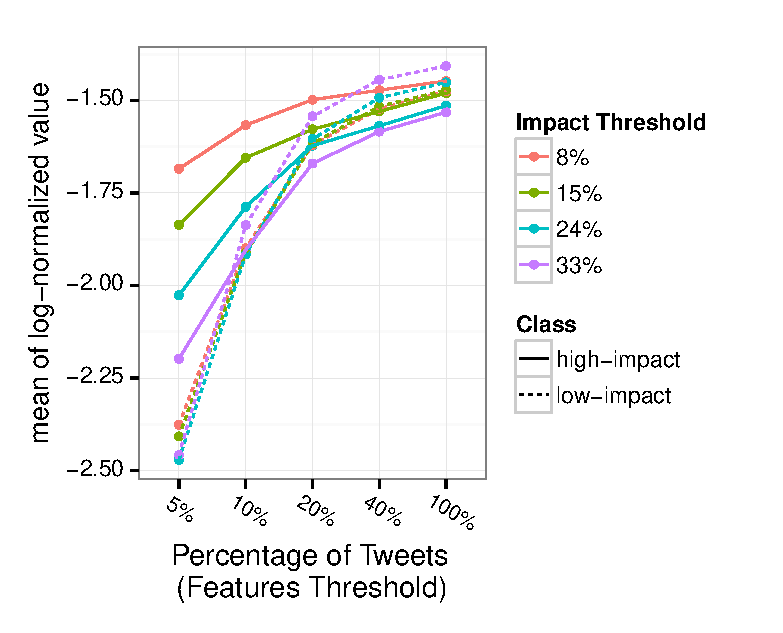
\includegraphics[width=\textwidth]{figures_SI/Plots_from_data/total_replies2.eps}
    \caption{Replies.} \label{fig:feat_replies}
  \end{subfigure}
  ~ %add desired spacing between images, e. g. ~, \quad, \qquad,
  % \hfill etc.
  % (or a blank line to force the subfigure onto a new line)
  \begin{subfigure}[b]{0.45\textwidth}
    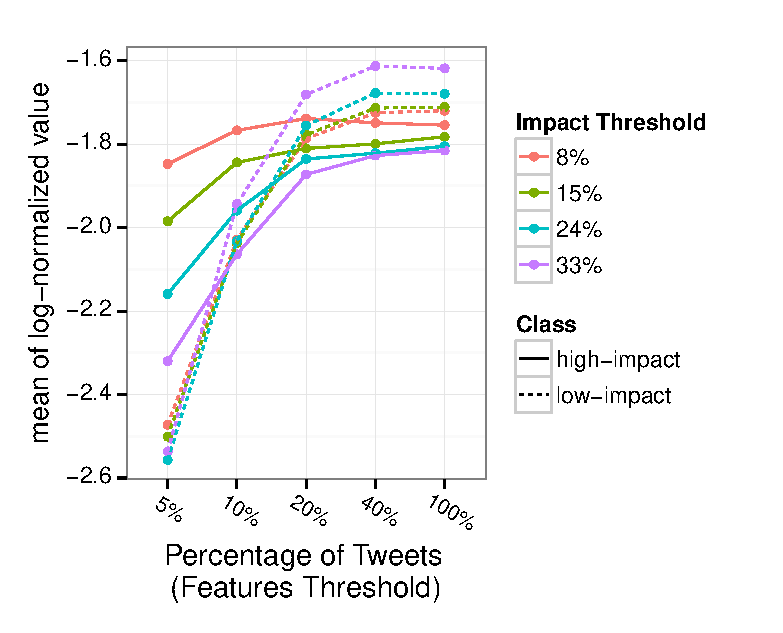
\includegraphics[width=\textwidth]{figures_SI/Plots_from_data/total_tweets_replied.eps}
    \caption{Tweets replied.} \label{fig:feat_tweets_replied}
  \end{subfigure} ~ %add desired spacing
  % between images, e. g. ~, \quad,
  % \qquad, \hfill etc. %(or a blank line
  % to force the subfigure onto a new
  % line)

  \begin{subfigure}[b]{0.45\textwidth}
    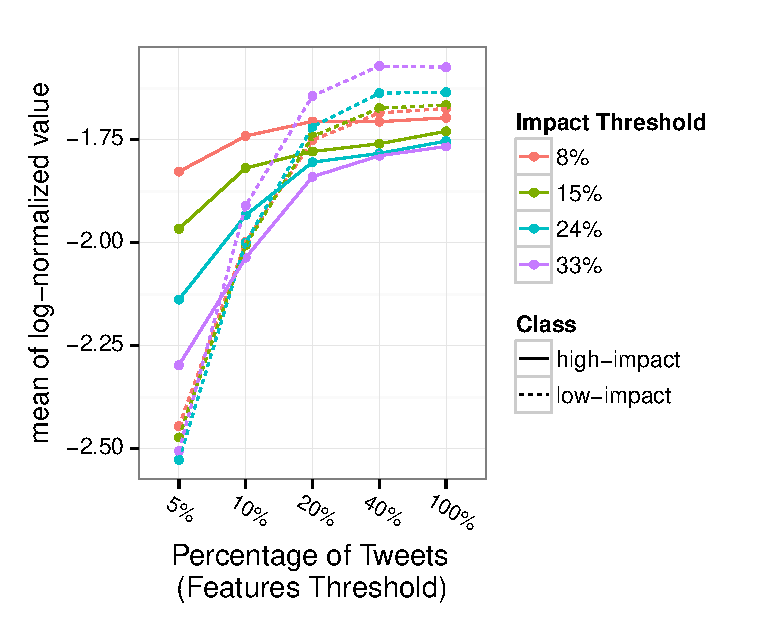
\includegraphics[width=\textwidth]{figures_SI/Plots_from_data/total_unique_users_replied.eps}
    \caption{Unique users
      replied.} \label{fig:feat_uniq_users_replied}
  \end{subfigure}
  \caption{\textbf{This figure illustrates how the features which
      explain the conversational hypothesis differ between the high
      impact and non-high impact events. The x-axis represents the
      progression of feature values as the event progresses. Each
      point on the graph represents the average value of the feature
      in all the high-impact and non-high impact events respectively.
      All solid lines represent high-impact events and all dashed
      lines represent non-high impact events. The different colors
      correspond to the results when the threshold of what is
      considered high-impact varies from the top 8\% to 33\%. }}
  \label{fig:conversational_hypothesis}
\end{figure}

% \begin{table}
%  \centering
%  {\small
%    \begin{tabular}{ll}
%      \toprule
%      Feature Name &  Description \\
%      \midrule
%      \texttt{replies} & \pbox{20cm}{$\log($total replies divided by total tweets$)$} \\
%      \midrule
%      \texttt{norm\_replies} & \pbox{20cm}{$\log($number of replies divided by total number of unique users$)$} \\
%      \midrule
%      \texttt{tweets\_replied} & \pbox{20cm}{$\log($number of tweets which generated replies divided by total tweets$)$} \\
%      \midrule
%      \texttt{uniq\_users\_replied} & \pbox{20cm}{$\log($unique users who have written a reply divided by total tweets$)$} \\
%      \bottomrule
%    \end{tabular}
%  }
%  \caption{\textbf{(Refer to Section~\ref{subsec:conversational}).
%      This table lists all the features which characterize the conversational aspect of events.}}
%  \label{tab:conversational}
%\end{table}
\subsection{Topical Focus Characteristics}
We find that high-impact events have a lot more focus in terms of the
topical content than low impact events. This intuitively makes sense
because when a news item is sensational, people seldom deviate from
the topic of the news to other things. We used four features listed in
Table~\ref{tab:topical_focus} to study the topic focus characteristics
of high-impact events.

\begin{table}
  \centering
  {\scriptsize
    \begin{tabular}{llll}
      \toprule
      Feature Name &  \multicolumn{1}{l}{Description} & High-impact, Non-high-impact value & Hypothesis, $p$-value\\
      \midrule
      \texttt{uniq\_words} & \pbox{20cm}{$\log($total unique words \\divided by total tweets$)$} & $-0.1982, 0.1651$ & $1$, $p = 0$ \\
      \midrule
      \texttt{uniq\_chars} & \pbox{20cm}{$\log($total unique characters \\divided by total tweets$)$} & $2.0009, 2.0456$ & $1$, $p = 0$ \\
      \midrule
      \texttt{uniq\_hashtags} & \pbox{20cm}{$\log($number of unique hashtags\\ divided by total tweets$)$} & $-1.1126, 0.8761$ & $1$, $p = 0$ \\
      \midrule
      \texttt{uniq\_urls} & \pbox{20cm}{$\log($number of unique urls \\divided by total tweets$)$} & $-0.7194, -0.4951$ & $1$, $p = 0$ \\
      \bottomrule
    \end{tabular}
  }
  \caption{\textbf{(Refer to Section~\ref{subsec:topical_focus}.)
      This table summarizes all the features that were used to study the topical focus characteristics
      of high-impact events.}}
  \label{tab:topical_focus}
\end{table}

The number of unique words (\texttt{uniq\_words}) and characters
(\texttt{uniq\_chars}) for high-impact events is lower than for low
impact events suggesting that the information content for high-impact
events is more focused than for low impact events (as they do not need
a diverse vocabulary). Hashtags on Twitter are a sequence of
characters that follow the \# symbol. Conventionally, their purpose is
to indicate the topic of the tweet. Again, this number
(\texttt{uniq\_hashtags}; log-normalized by the total number of
tweets) is lower for the high-impact events than for the low impact
ones. The number of unique URLs (\texttt{uniq\_urls}; which can be
taken to interpret similar semantics as the hashtags) is also lower
for high-impact events than for the rest. 

Figure~\ref{fig:topical_focus_hypothesis} comprehensively illustrates
all the features associated with the topical focus characteristics of
the event through all the phases. Note that for all features, a lower
value indicates a greater focus on the topic at hand. From the plots,
we can infer that high-impact events, through all the phases have a
higher topical focus than their non-high impact counter parts. For example,
\texttt{uniq\_hashtags} has a general downward trend over time. It turns
out that invention of the hashtags mostly takes place in the first
phase of the event. As the event evolves in time, even though the
total number of tweets grow, the raw number of the unique hashtags
does not increase at the same rate.
\label{subsec:topical_focus}
\begin{figure}[h]
  \centering
  \begin{subfigure}[h]{0.45\textwidth}
    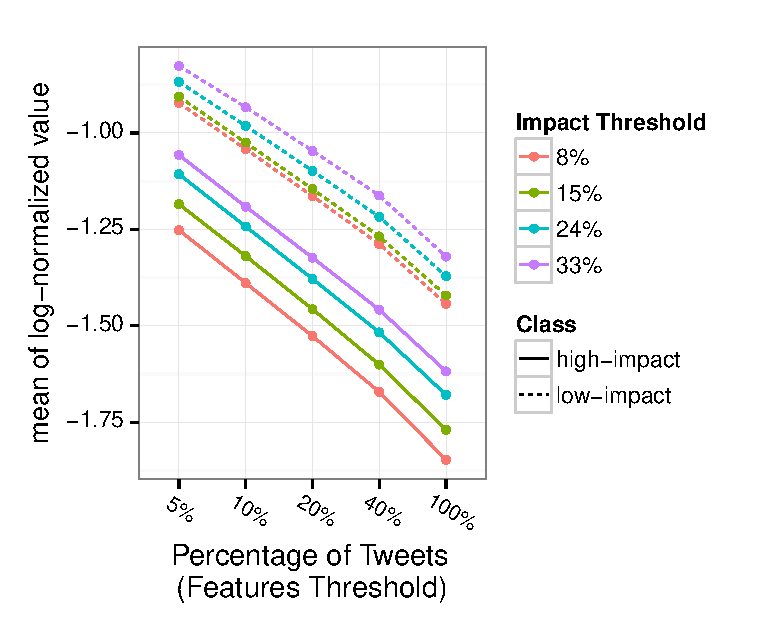
\includegraphics[width=\textwidth]{figures_SI/Plots_from_data/total_unique_words.eps}
    \caption{Unique words.} \label{fig:feat_uniq_words}
  \end{subfigure}
  ~ %add desired spacing between images, e. g. ~, \quad, \qquad,
  % \hfill etc.
  % (or a blank line to force the subfigure onto a new line)
  \begin{subfigure}[h]{0.45\textwidth}
    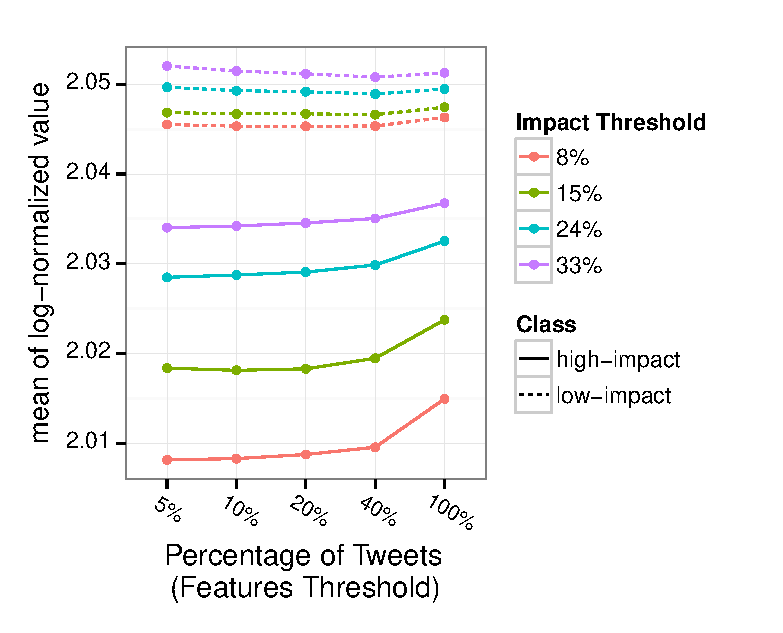
\includegraphics[width=\textwidth]{figures_SI/Plots_from_data/total_characters.eps}
    \caption{Total characters.} \label{fig:feat_characters}
  \end{subfigure} ~ %add desired spacing
  % between images, e. g. ~, \quad,
  % \qquad, \hfill etc. %(or a blank line
  % to force the subfigure onto a new
  % line)

  \begin{subfigure}[h]{0.45\textwidth}
    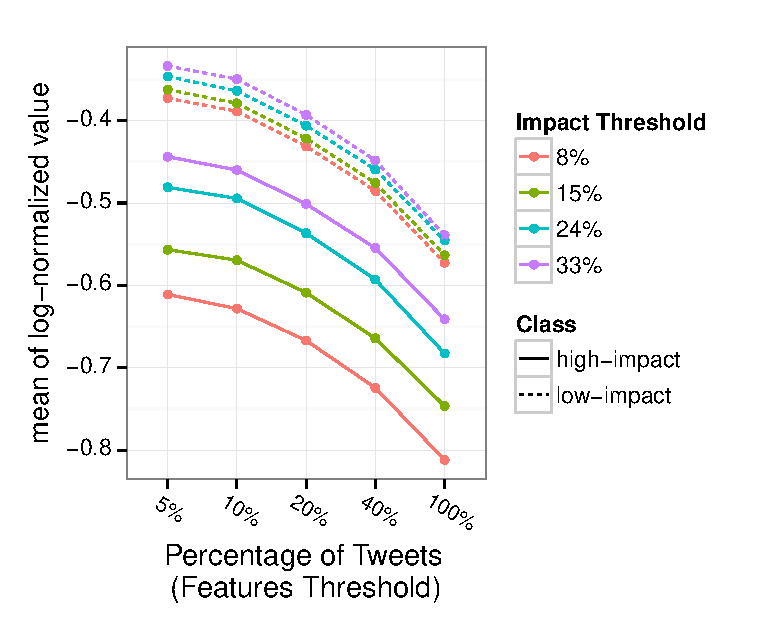
\includegraphics[width=\textwidth]{figures_SI/Plots_from_data/total_unique_hashtags.eps}
    \caption{Unique hashtags.} \label{fig:feat_uniq_hashtags}
  \end{subfigure}
  ~
  \begin{subfigure}[h]{0.45\textwidth}
    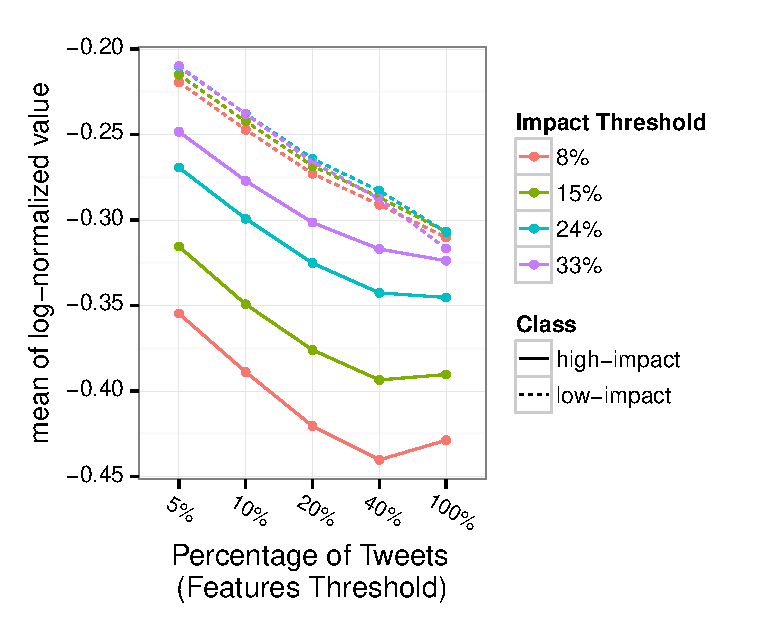
\includegraphics[width=\textwidth]{figures_SI/Plots_from_data/total_unique_urls.eps}
    \caption{Unique URLs.} \label{fig:feat_uniq_urls}
  \end{subfigure}
  \caption{\textbf{This figure illustrates how the features which
      explain the topical focus characteristics differ between the
      high-impact and non-high impact events. The x-axis represents
      the progression of feature values as the event progresses. Each
      point on the graph represents the average value of the feature
      in all the high-impact and non-high impact events respectively.
      All solid lines represent high-impact events and all dashed
      lines represent non-high impact events. The different colors
      correspond to the results when the threshold of what is
      considered high-impact varies from the top 8\% to 33\%. }}
  \label{fig:topical_focus_hypothesis}
\end{figure}

% \begin{table}
%  \centering
%  {\small
%    \begin{tabular}{ll}
%      \toprule
%      Feature Name &  Description\\
%      \midrule
%      \texttt{uniq\_words} & \pbox{20cm}{$\log($total unique words divided by total tweets$)$}\\
%      \midrule
%      \texttt{uniq\_chars} & \pbox{20cm}{$\log($total unique characters divided by total tweets$)$}\\
%      \midrule
%      \texttt{uniq\_hashtags} & \pbox{20cm}{$\log($number of unique hashtags divided by total tweets$)$}\\
%      \midrule
%      \texttt{uniq\_urls} & \pbox{20cm}{$\log($number of unique urls divided by total tweets$)$}\\
%      \bottomrule
%    \end{tabular}
%  }
%  \caption{\textbf{(Refer to Section~\ref{subsec:topical_focus}).
%      This table summarizes all the features that were used to study the topical focus characteristics
%      of high-impact events.}}
%  \label{tab:topical_focus}
%\end{table}
\subsection{Classification of high-impact Events}
\label{subsec:classification}
Figure~\ref{fig:classification} illustrates the classification results
of high-impact events across all thresholds and through all phases of
the event, and Tables~\ref{tab:confusion_matrix}
and~\ref{tab:classification_results} encapsulate the prediction results
from the early tweets, while predicting the top 8\% high-impact
events. We note that in all the plots, the false positive rate is 
10\% or less. We also note that the precision and ROC-area both are
consistently above 80\% and remain more or less the same through all
the plots. However, there is a gradual increase in the recall value as
it evolves and also as the threshold varies. The recall value
increasing as the event evolves suggests that some high-impact events
perhaps do not start displaying their ``high impact'' characteristics
well enough in their early stages. In some sense, they are the late
bloomers. This prevents them from being detected from the early tweets
about these events. As we vary the threshold from 8\% to 33\%, we are
becoming less and less stringent about what we consider to be
high-impact events. This perhaps helps in detecting those events which
are the late bloomers, and yields a higher recall value.
\begin{figure}
  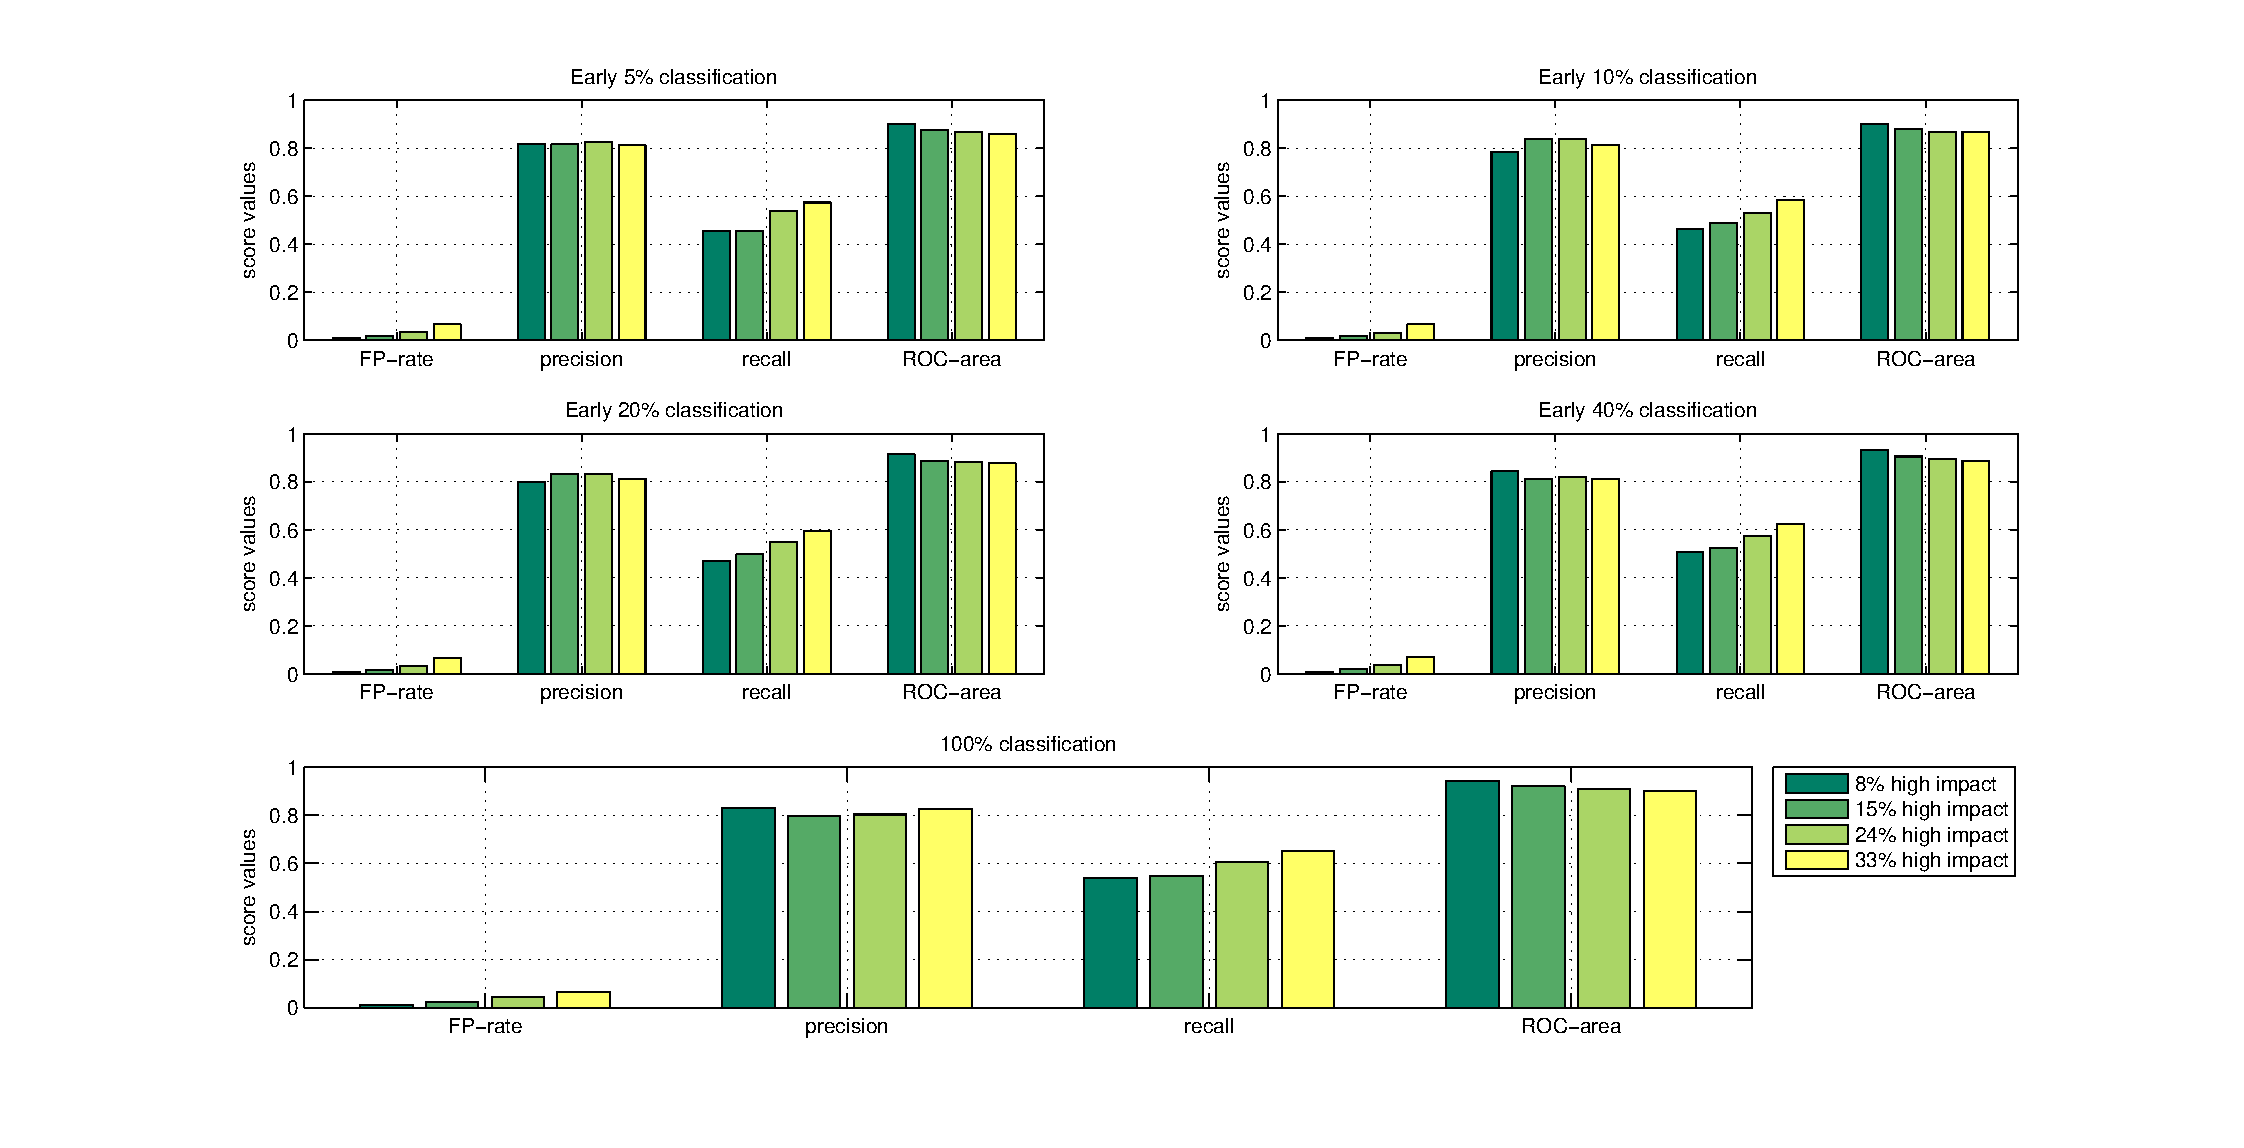
\includegraphics[width=\textwidth]{figures_SI/Plots_from_data/comprehensive_classification}
  \caption{\textbf{This figure illustrates the classification results
      of high-impact events across all thresholds, and through all
      phases of the event.}}
  \label{fig:classification}
\end{figure}

\begin{table}
  \centering
  % {\scriptsize
  \begin{tabular}{lcc|cc}
    \toprule
    \multirow{2}{*}{ }& \multicolumn{2}{c}{Early 5\% Tweets} & \multicolumn{2}{c}{All Tweets} \\
    \midrule
    % \cmidrule{2-5} \cline{2-5}
    & high-impact & non-high-impact & high-impact & non-high-impact \\
    % \midrule
    high-impact & $194$ & $232$ & $230$ & $196$\\
    non-high-impact & $43$ & $4\,765$ & $47$ & $4\,761$ \\
    \bottomrule
  \end{tabular}
  % }
  \caption{\textbf{Confusion matrix while predicting the top 8\% of events
      as high-impact.  The predictions were made using the early 5\% of the tweets, and by using
      all the tweets from the event.}}
  \label{tab:confusion_matrix}
\end{table}
\begin{table}

  \centering
  {\small
    \begin{tabular}{lcccc|cccc}
      \toprule
      & \multicolumn{4}{c}{Early 5\% Tweets} & \multicolumn{4}{c}{All Tweets} \\
      \midrule
      & FP-Rate & Precision & Recall & ROC-area & FP-Rate & Precision & Recall & ROC-area \\
      % \midrule
      high-impact & 0.009 & 0.819 & 0.455 & 0.900 & 0.01 & 0.830 & 0.540 & 0.945 \\
      non-high-impact & 0.545 & 0.954 & 0.991 & 0.900 &  0.460 & 0.960 & 0.990 & 0.945 \\
      \bottomrule
    \end{tabular}
  }
  \caption{\textbf{Classification results of detecting whether an event from the top 8\% is high-impact or not
      while predicting from features extracted from the earliest 5\% of the tweets and from all the tweets belonging to the event.}}
  \label{tab:classification_results}
\end{table}

\subsection{Features used for analysis}

Table~\ref{tab:feats} shows a list of the features used for the
characterization and classification of news events, along with the
normalization method used.

{\footnotesize
  \begin{longtable}{l|l|l}

    \hline \textbf{Feature Name} & \textbf{Normalized By} &
    \textbf{Normalization
      Method} \\
    \hline
    \endfirsthead
    \multicolumn{3}{l}%
    {\tablename\ \thetable\ -- \textit{Continued from previous page}} \\
    \hline \textbf{Feature Name} & \textbf{Normalized By} &
    \textbf{Normalization
      Method} \\
    \hline
    \endhead
    \hline \multicolumn{3}{l}{\textit{Continued on next page}} \\
    \endfoot
    \hline
    \endlastfoot


    \texttt{component\_size}	&	 None	&	  \\
    \texttt{total\_seconds}	&	 \texttt{total\_tweets}	& $\log(x) - \log(y)$ \\
    \texttt{total\_tweets}	&	 None	&	  \\
    \texttt{total\_retweets}	&	 \texttt{total\_tweets}	&	 $\log(x) - \log(y)$ \\
    \texttt{total\_tweets\_retweeted}	&	 \texttt{total\_tweets}	&	 $\log(x) - \log(y)$ \\
    \texttt{retweets\_most\_retweeted}	&	 \texttt{total\_retweets}	&	 $\log(x) - \log(y)$ \\
    \texttt{total\_mentions}	&	 \texttt{total\_tweets}	&	 $\log(x) - \log(y)$ \\
    \texttt{total\_unique\_mentions} &
    \texttt{total\_mentions}	&	 $\log(x) - \log(y)$ \\
    \texttt{total\_tweets\_with\_mention}	&	 \texttt{total\_tweets}	&	 $\log(x) - \log(y)$ \\
    \texttt{total\_tweets\_with\_mostfrequent\_mention}	&	 \texttt{total\_tweets\_with\_mention}	&	 $\log(x) - \log(y)$ \\
    \texttt{total\_hashtags}	&	 \texttt{total\_tweets}	&	 $\log(x) - \log(y)$ \\
    \texttt{total\_unique\_hashtags}	&	 \texttt{total\_hashtags}	&	 $\log(x) - \log(y)$ \\
    \texttt{total\_tweets\_with\_hashtag}	&	 \texttt{total\_tweets}	&	 $\log(x) - \log(y)$ \\
    \texttt{total\_tweets\_with\_mostfrequent\_hashtag}	&	 \texttt{total\_tweets\_with\_hashtag}	&	 $\log(x) - \log(y)$ \\
    \texttt{total\_urls}	&	 \texttt{total\_tweets}	&	 $\log(x) - \log(y)$ \\
    \texttt{total\_unique\_urls}	&	 \texttt{total\_urls}	&	 $\log(x) - \log(y)$ \\
    \texttt{total\_tweets\_with\_url}	&	 \texttt{total\_tweets}	&	 $\log(x) - \log(y)$ \\
    \texttt{total\_tweets\_with\_mostfrequent\_url}	&	 \texttt{total\_tweets\_with\_url}	&	 $\log(x) - \log(y)$ \\
    \texttt{total\_unique\_verified\_users}	&	 \texttt{total\_verified\_users}	&	 $\log(x) - \log(y)$ \\
    \texttt{total\_verified\_users}	&	 \texttt{total\_tweets}	&	 $\log(x) - \log(y)$ \\
    \texttt{total\_unique\_users}	&	 \texttt{total\_tweets}	&	 $\log(x) - \log(y)$ \\
    \texttt{total\_replies} & \texttt{total\_unique\_users} &
    $\log(x) - \log(y)$ \\
    \texttt{total\_tweets\_first\_replied} & \texttt{total\_tweets} &
    $\log(x) - \log(y)$ \\
    \texttt{total\_unique\_users\_replied} &
    \texttt{total\_unique\_users} &
    $\log(x) - \log(y)$ \\
    \texttt{total\_tweets\_replied}	&	 \texttt{total\_tweets}	&	 $\log(x) - \log(y)$ \\
    \texttt{total\_words}	&	 \texttt{total\_tweets}	&	 $\log(x) - \log(y)$ \\
    \texttt{total\_unique\_words}	&	 \texttt{total\_words}	&	 $\log(x) - \log(y)$ \\
    \texttt{total\_characters}	&	 \texttt{total\_tweets}	&	 $\log(x) - \log(y)$ \\
    \texttt{total\_rt\_count}	&	 \texttt{total\_tweets}	&	 $\log(x) - \log(y)$ \\
    \texttt{total\_fav\_count}	&	 \texttt{total\_tweets}	&	 $\log(x) - \log(y)$ \\
    \texttt{total\_positive\_sentiment}	& \texttt{total\_tweets}	&	 $x / y$ \\
    \texttt{total\_negative\_sentiment}	&	 \texttt{total\_tweets}	&	 $x / y$ \\
    \hline

    \caption[List of features used for characterization]{\textbf{List
        of features used for characterization and classification. The
        ``Normalization Method'' column corresponds to the method used
        to normalize the value of the first column using the value of
        the second column. For example, the total number of retweets
        was normalized dividing it by the total number of tweets, and
        then taking the logarithm. Zero values were replaced by
        $10^{-8}$.}}
    \label{tab:feats}
  \end{longtable}

